%%%%%%%%%%%%%%%%%%%%%%%%%%%%%%%%%%%%%%%%%%%%%%%%%%%%%%%%%%%%%%%%%%%%%%%%%%%
%%
%% Filename: 	spec.tex
%%
%% Project:	Zip CPU -- a small, lightweight, RISC CPU soft core
%%
%% Purpose:	This LaTeX file contains all of the documentation/description
%%		currently provided with this Zip CPU soft core.  It supersedes
%%		any information about the instruction set or CPUs found
%%		elsewhere.  It's not nearly as interesting, though, as the PDF
%%		file it creates, so I'd recommend reading that before diving
%%		into this file.  You should be able to find the PDF file in
%%		the SVN distribution together with this PDF file and a copy of
%%		the GPL-3.0 license this file is distributed under.  If not,
%%		just type 'make' in the doc directory and it (should) build
%%		without a problem.
%%		
%%
%% Creator:	Dan Gisselquist
%%		Gisselquist Technology, LLC
%%
%%%%%%%%%%%%%%%%%%%%%%%%%%%%%%%%%%%%%%%%%%%%%%%%%%%%%%%%%%%%%%%%%%%%%%%%%%%
%%
%% Copyright (C) 2015, Gisselquist Technology, LLC
%%
%% This program is free software (firmware): you can redistribute it and/or
%% modify it under the terms of  the GNU General Public License as published
%% by the Free Software Foundation, either version 3 of the License, or (at
%% your option) any later version.
%%
%% This program is distributed in the hope that it will be useful, but WITHOUT
%% ANY WARRANTY; without even the implied warranty of MERCHANTIBILITY or
%% FITNESS FOR A PARTICULAR PURPOSE.  See the GNU General Public License
%% for more details.
%%
%% You should have received a copy of the GNU General Public License along
%% with this program.  (It's in the $(ROOT)/doc directory, run make with no
%% target there if the PDF file isn't present.)  If not, see
%% <http://www.gnu.org/licenses/> for a copy.
%%
%% License:	GPL, v3, as defined and found on www.gnu.org,
%%		http://www.gnu.org/licenses/gpl.html
%%
%%
%%%%%%%%%%%%%%%%%%%%%%%%%%%%%%%%%%%%%%%%%%%%%%%%%%%%%%%%%%%%%%%%%%%%%%%%%%%
%
%
%
% From TI about DSPs vs FPGAs:
%	www.ti.com/general/docs/video/foldersGallery.tsp?bkg=gray
%	&gpn=35145&familyid=1622&keyMatch=DSP Breaktime Episode Three
%	&tisearch=Search-EN-Everything&DCMP=leadership
%	&HQS=ep-pro-dsp-leadership-problog-150518-v-en
%
%	FPGA's are annoyingly faster, cheaper, and not quite as power hungry
%	as they used to be.
%
%	Why would you choose DSPs over FPGAs?  If you care about size,
%	if you care about power, or happen to have a complicated algorithm
%	that just isn't simply doing the same thing over and over
%
%	For complex algorithms that change over time.  Each have their strengths
%	sometimes you can use both.
%
%	"No assembly required" -- TI tools all C programming, very GUI based
%	environment, very little optimization by hand ...
%
%
% The FPGA's achilles heel: Reconfigurability.  It is very difficult, although
% I'm sure major vendors will tell you not impossible, to reconfigure an FPGA
% based upon the need to process time-sensitive data.  If you need one of two
% algorithms, both which will fit on the FPGA individually but not together,
% switching between them on the fly is next to impossible, whereas switching
% algorithm within a CPU is not difficult at all.  For example, imagine 
% receiving a packet and needing to apply one of two data algorithms on the
% packet before sending it back out, and needing to do so fast.  If both
% algorithms don't fit in memory, where does the packet go when you need to
% swap one algorithm out for the other?  And what is the cost of that "context"
% swap?
%
%
\documentclass{gqtekspec}
\usepackage{import}
\usepackage{bytefield}	% Install via apt-get install texlive-science
% \graphicspath{{../gfx}}
\project{Zip CPU}
\title{Specification}
\author{Dan Gisselquist, Ph.D.}
\email{dgisselq (at) opencores.org}
\revision{Rev.~0.91}
\definecolor{webred}{rgb}{0.5,0,0}
\definecolor{webgreen}{rgb}{0,0.4,0}
\hypersetup{
	ps2pdf,
	pdfpagelabels,
	hypertexnames,
	pdfauthor={Dan Gisselquist},
	pdfsubject={Zip CPU},
	anchorcolor= black,
	colorlinks = true,
	linkcolor  = webred,
	citecolor  = webgreen
}
\begin{document}
\pagestyle{gqtekspecplain}
\titlepage
\begin{license}
Copyright (C) \theyear\today, Gisselquist Technology, LLC

This project is free software (firmware): you can redistribute it and/or
modify it under the terms of  the GNU General Public License as published
by the Free Software Foundation, either version 3 of the License, or (at
your option) any later version.

This program is distributed in the hope that it will be useful, but WITHOUT
ANY WARRANTY; without even the implied warranty of MERCHANTIBILITY or
FITNESS FOR A PARTICULAR PURPOSE.  See the GNU General Public License
for more details.

You should have received a copy of the GNU General Public License along
with this program.  If not, see \hbox{<http://www.gnu.org/licenses/>} for a
copy.
\end{license}
\begin{revisionhistory}
0.9 & 4/20/2016 & Gisselquist & Modified ISA: LDIHI replaced with MPY, MPYU and MPYS replaced with MPYUHI, and MPYSHI respectively.  LOCK instruction now
permits an intermediate ALU operation. \\\hline
0.91& 7/16/2016 & Gisselquist & :escribed three more CC bits\\\hline
0.8 & 1/28/2016 & Gisselquist & Reduced complexity early branching \\\hline
0.7 & 12/22/2015 & Gisselquist & New Instruction Set Architecture \\\hline
0.6 & 11/17/2015 & Gisselquist & Added graphics to illustrate pipeline discussion.\\\hline
0.5 & 9/29/2015 & Gisselquist & Added pipelined memory access discussion.\\\hline
0.4 & 9/19/2015 & Gisselquist & Added DMA controller, improved stall information, and self--assessment info.\\\hline
0.3 & 8/22/2015 & Gisselquist & First completed draft\\\hline
0.2 & 8/19/2015 & Gisselquist & Still Draft, more complete \\\hline
0.1 & 8/17/2015 & Gisselquist & Incomplete First Draft \\\hline
\end{revisionhistory}
% Revision History
% Table of Contents, named Contents
\tableofcontents
\listoffigures
\listoftables
\begin{preface}
Many people have asked me why I am building the Zip CPU. ARM processors are
good and effective. Xilinx makes and markets Microblaze, Altera Nios, and both
have better toolsets than the Zip CPU will ever have. OpenRISC is also
available, RISC--V may be replacing it. Why build a new processor?

The easiest, most obvious answer is the simple one: Because I can.

There's more to it, though. There's a lot that I would like to do with a
processor, and I want to be able to do it in a vendor independent fashion.
First, I would like to be able to place this processor inside an FPGA.  Without
paying royalties, ARM is out of the question.  I would then like to be able to
generate Verilog code, both for the processor and the system it sits within,
that can run equivalently on both Xilinx and Altera chips, and that can be
easily ported from one manufacturer's chipsets to another. Even more, before
purchasing a chip or a board, I would like to know that my soft core works. I
would like to build a test bench to test components with, and Verilator is my
chosen test bench. This forces me to use all Verilog, and it prevents me from
using any proprietary cores. For this reason, Microblaze and Nios are out of
the question.

Why not OpenRISC? That's a hard question. The OpenRISC team has done some
wonderful work on an amazing processor, and I'll have to admit that I am
envious of what they've accomplished. I would like to port GDB to the
Zip CPU, give it an MMU, and then get Linux running on it. Indeed, the
OpenRISC team is are way ahead of me. The OpenRISC processor, however, is
complex and hefty at about 4,500 LUTs--and this without even implementing all
of their instructions. It has a lot of features of modern CPUs within it
that ... well, let's just say it's not the little guy on the block. The
Zip CPU on the other hand is lighter weight, costing only about 2,200~LUTs
with no peripherals, and 3,200~LUTs with some very basic peripherals.

My final reason is that I'm building the Zip CPU as a learning experience. The
Zip CPU has allowed me to learn a lot about how CPUs work on a very micro
level. For the first time, I am beginning to understand many of the Computer
Architecture lessons from years ago.

To summarize: Because I can, because it is open source, because it is light
weight, and as an exercise in learning. 

\end{preface}

\chapter{Introduction}
\pagenumbering{arabic}
\setcounter{page}{1}

The original goal of the Zip CPU was to be a very simple CPU.   You might
think of it as a poor man's alternative to the OpenRISC architecture.
For this reason, all instructions have been designed to be as simple as
possible, and the base instructions are all designed to be executed in one
instruction cycle per instruction, barring pipeline stalls.  Indeed, even the
bus has been simplified to a constant 32-bit width, with no option for more
or less.  This has resulted in the choice to drop push and pop instructions,
pre-increment and post-decrement addressing modes, and more.

For those who like buzz words, the Zip CPU is:
\begin{itemize}
\item A 32-bit CPU: All registers are 32-bits, addresses are 32-bits,
		instructions are 32-bits wide, etc.  Indeed, the ``byte size''
		for this processor, as per the C--language definition of a
		``byte'' is 32--bits.
\item A RISC CPU.  There is no microcode for executing instructions.  All
	instructions are designed to be completed in one clock cycle.
\item A Load/Store architecture.  (Only load and store instructions
		can access memory.)
\item Wishbone compliant.  All peripherals are accessed just like
		memory across this bus.
\item A Von-Neumann architecture.  (The instructions and data share a 
		common bus.)
\item A pipelined architecture, having stages for {\bf Prefetch},
	{\bf Decode}, {\bf Read-Operand}, a combined stage containing
	the {\bf ALU}, {\bf Memory}, {\bf Divide}, and {\bf Floating Point}
	units, and then the final {\bf Write-back} stage. 
		See Fig.~\ref{fig:cpu}
\begin{figure}\begin{center}
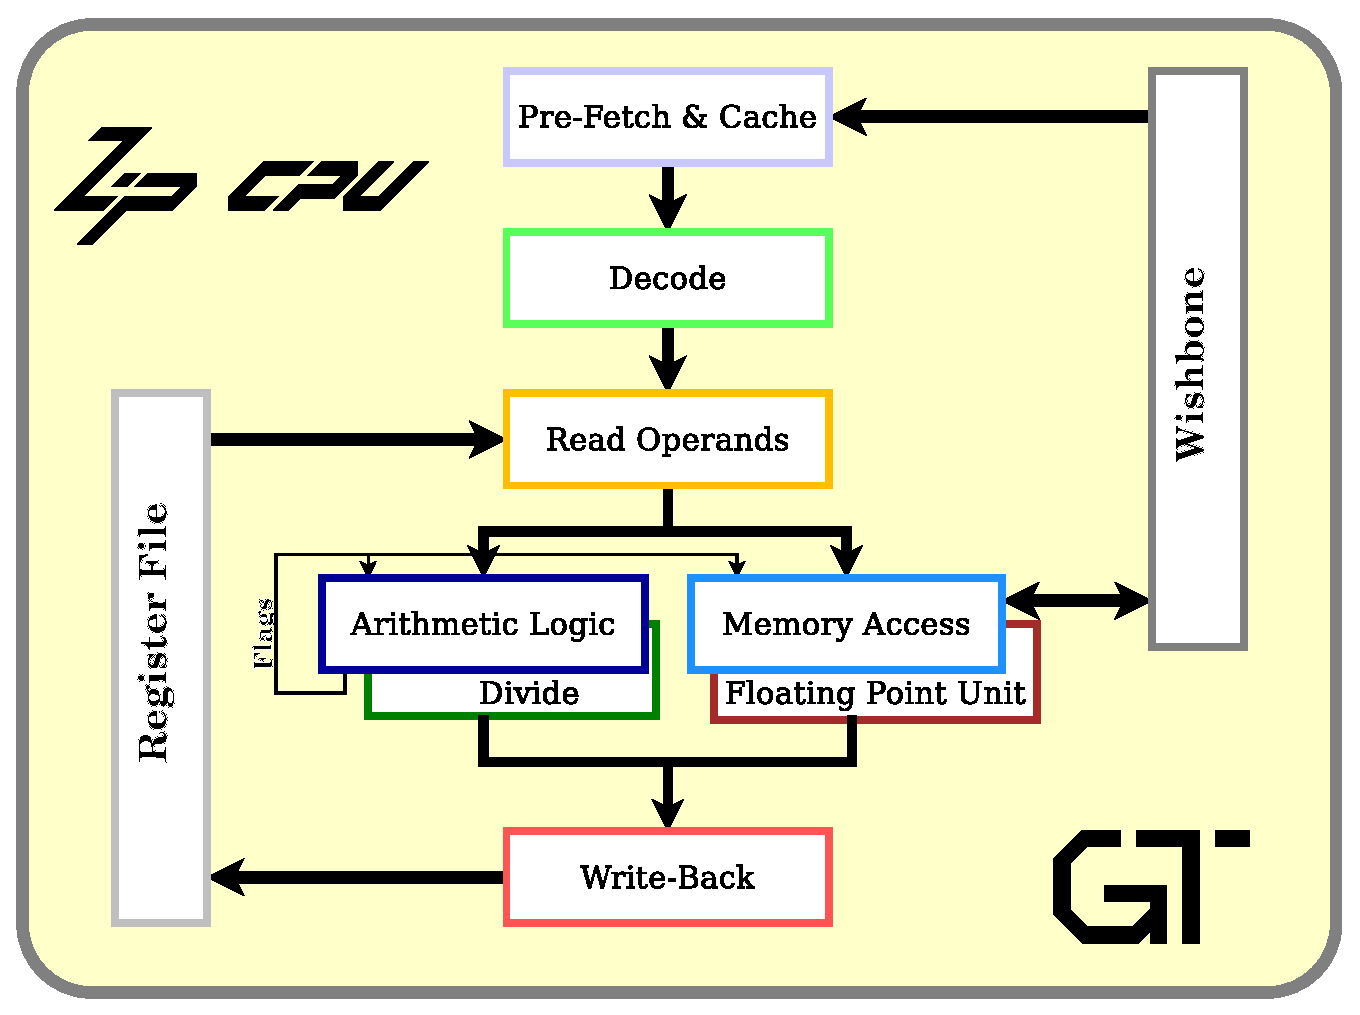
\includegraphics[width=3.5in]{../gfx/cpu.eps}
\caption{Zip CPU internal pipeline architecture}\label{fig:cpu}
\end{center}\end{figure}
		for a diagram of this structure.
\item Completely open source, licensed under the GPL.\footnote{Should you
	need a copy of the Zip CPU licensed under other terms, please 
	contact me.}
\end{itemize}

The Zip CPU also has one very unique feature: the ability to do pipelined loads
and stores.  This allows the CPU to access on-chip memory at one access per
clock, minus any stalls for the initial access.

\section{Characteristics of a SwiC}

Many other FPGA processors have been defined to be good Systems on a Chip, or 
SoC's.  The entire goal of the chip, then, is to provide an interface to the
processor and its external environment.  This is not the case with the Zip
CPU.  Instead, we shall define a new concept, that of a soft core internal to
an FPGA, as a ``System within a Chip,'' or a SwiC.  SwiCs have some very
unique properties internal to them that have influenced the design of the
Zip CPU.  Among these are the bus, memory, and available peripherals.

Many other approaches to soft core CPU's employ a Harvard architecture. 
This allows these other CPU's to have two separate bus structures: one for the
program fetch, and the other for the memory.  The Zip CPU is fairly unique in
its approach because it uses a von Neumann architecture. 
By using a von Neumann architecture, only one bus needs to be implemented
within any FPGA.  This was structure was chosen for simplicity. 
Having only the one bus helps to minimize real-estate, while
maintaining a high clock speed.  The disadvantage is that it can severely
degrade the overall instructions per clock count when the prefetch and
memory access unit both want access to the bus.

Soft core's within an FPGA have an additional characteristic regarding
memory access: it is slow.  While memory on chip may be accessed at a single
cycle per access, small FPGA's often have only a limited amount of memory on
chip.  Going off chip, however, is expensive.  Two examples will prove this
point.  On
the XuLA2 board, Flash can be accessed at 128~cycles per 32--bit word,
or 64~cycles per subsequent word in a pipelined architecture.  Likewise, the
SDRAM chip on the XuLA2 board allows a 6~cycle access for a write, 10~cycles
per read, and 2~cycles for any subsequent pipelined access read or write.
Either way you look at it, this memory access will be slow and this doesn't
account for any logic delays should the bus implementation logic get
complicated.

As may be noticed from the above discussion about memory speed, a second
characteristic of memory is sequential memory accesses may be optimized for
minimal delays (pipelined), and that pipelined memory access is faster than
non--pipelined access.  Therefore, a SwiC soft core should support pipelined
operations, but it should also allow a higher priority subsystem to get access
to the bus (no starvation).

As a further characteristic of SwiC memory options, on-chip cache's are
expensive.  If you want to have a minimum of logic, cache logic may not be
the highest on the priority list.

In sum, memory is slow.  While one processor on one FPGA may be able to fill
its pipeline, the same processor on another FPGA may struggle to get more than
one instruction at a time into the pipeline.  Any SwiC must be able to deal
with both cases: fast and slow memories.

A final characteristic of SwiC's within FPGA's is the peripherals. 
Specifically, FPGA's are highly reconfigurable.  Soft peripherals can easily
be created on chip to support the SwiC if necessary.  As an example, a simple
30-bit peripheral could easily support reversing 30-bit numbers: a read from
the peripheral returns it's bit--reversed address.  This is cheap within an
FPGA, but expensive in instructions.  Reading from another 16--bit peripheral
might calculate a sine function, where the 16--bit address internal to the
peripheral was the angle of the sine wave.

Indeed, anything that must be done fast within an FPGA is likely to already
be done--elsewhere in the fabric.  This leaves the CPU with the simple role
of solely handling sequential tasks that need a lot of state.

This means that the SwiC needs to live within a very unique environment,
separate and different from the traditional SoC.  That isn't to say that a 
SwiC cannot be turned into a SoC, just that this SwiC has not been designed
for that purpose.

\section{Lessons Learned}

Now, however, that I've worked on the Zip CPU for a while, it is not nearly
as simple as I originally hoped.  Worse, I've had to adjust to create
capabilities that I was never expecting to need.  These include:
\begin{itemize}
\item {\bf External Debug:} Once placed upon an FPGA, some external means is
	still necessary to debug this CPU.  That means that there needs to be
	an external register that can control the CPU: reset it, halt it, step
	it, and tell whether it is running or not.  My chosen interface
	includes a second register similar to this control register.  This
	second register allows the external controller or debugger to examine
	registers internal to the CPU.

\item {\bf Internal Debug:} Being able to run a debugger from within
	a user process requires an ability to step a user process from
	within a debugger.  It also requires a break instruction that can
	be substituted for any other instruction, and substituted back.
	The break is actually quite difficult: the break instruction cannot be
	allowed to execute.  That way, upon a break, the debugger should
	be able to jump back into the user process to step the instruction
	that would've been at the break point initially, and then to 
	replace the break after passing it.

	Incidentally, this break messes with the prefetch cache and the
	pipeline: if you change an instruction partially through the pipeline,
	the whole pipeline needs to be cleansed.  Likewise if you change
	an instruction in memory, you need to make sure the cache is reloaded
	with the new instruction.

\item {\bf Prefetch Cache:} My original implementation, {\tt prefetch}, had
	a very simple prefetch stage.  Any time the PC changed the prefetch
	would go and fetch the new instruction.  While this was perhaps this
	simplest approach, it cost roughly five clocks for every instruction. 
	This was deemed unacceptable, as I wanted a CPU that could execute
	instructions in one cycle. 

	My second implementation, {\tt pipefetch}, attempted to maximize its
	use of pipelined memory.  When a new CPU address was issued, it would
	start reading memory in a pipelined fashion, and issuing instructions
	as soon as they were ready.  The result was a cache that was
	conceptually just a sliding window in memory.  This suffered
	from some difficult performance problems, though.  If the CPU was
	alternating between two diverse sections of code, both could never be
	in the cache at the same time--causing lots of cache misses.  Further,
	the extra logic to implement this window cost an extra clock cycle
	in the cache implementation, slowing down branches.

	The Zip CPU now has a third cache implementation, {\tt pfcache}.  This
	new implementation takes only a single cycle per access, but costs a
	full cache line miss on any miss.  While configurable, a full cache
	line miss might mean that the CPU needs to read 256~instructions from
	memory before it can execute the first one of them.

\item {\bf Operating System:} In order to support an operating system,
	interrupts and so forth, the CPU needs to support supervisor and
	user modes, as well as a means of switching between them.  For example,
	the user needs a means of executing a system call.  This is the 
	purpose of the {\bf `trap'} instruction.  This instruction needs to
	place the CPU into supervisor mode (here equivalent to disabling
	interrupts), as well as handing it a parameter such as identifying
	which O/S function was called. 

	My initial approach to building a trap instruction was to create an
	external peripheral which, when written to, would generate an
	interrupt and could return the last value written to it.  In practice,
	this approach didn't work at all: the CPU executed two instructions
	while waiting for the trap interrupt to take place.  Since then, I've
	decided to keep the rest of the CC register for that purpose so that
	a write to the CC register, with the GIE bit cleared, could be used
	to execute a trap.  This has other problems, though, primarily in the
	limitation of the uses of the CC register.  In particular, the CC
	register is the best place to put CPU state information and to
	``announce'' special CPU features (floating point, etc).  So the trap
	instruction still switches to interrupt mode, but the CC register is not
	nearly as useful for telling the supervisor mode processor what trap
	is being executed.

	Modern timesharing systems also depend upon a {\bf Timer} interrupt
	to handle task swapping.  For the Zip CPU, this interrupt is handled
	external to the CPU as part of the CPU System, found in
	{\tt zipsystem.v}.  Small area implementations might find this
	peripheral package too expensive, however, so the timer module itself
	is found in {\tt ziptimer.v} and may be implemented as needed with
	the CPU.

\item {\bf Bus Errors:} My original implementation had no logic to handle
	what would happen if the CPU attempted to read or write a non-existent
	memory address.  This changed after I needed to troubleshoot a failure
	caused by a subroutine return to a non-existent address.

	My next problem bus problem was caused by a misbehaving peripheral.
	Whenever the CPU attempted to read from or write to this peripheral,
	the peripheral would take control of the wishbone bus and not return
	it.  For example, it might never return an {\tt ACK} to signal
	the end of the bus transaction.  This led to the implementation of
	a wishbone bus watchdog that would create a bus error if any particular
	bus action didn't complete in a timely fashion.

\item {\bf Pipeline Stalls:} My original plan was to not support pipeline
	stalls at all, but rather to require the compiler to properly schedule
	all instructions so that stalls would never be necessary.  After trying
	to build such an architecture, I gave up, having learned some things:

	First, and ideal pipeline might look something like
	Fig.~\ref{fig:ideal-pipeline}.
\begin{figure}
\begin{center}
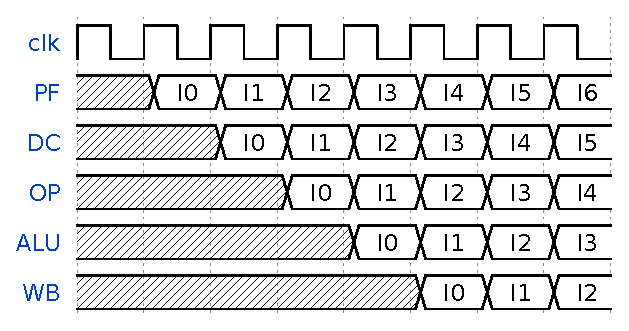
\includegraphics[width=4in]{../gfx/fullpline.eps}
\caption{An Ideal Pipeline: One instruction per clock cycle}\label{fig:ideal-pipeline}
\end{center}\end{figure}
	Notice that, in this figure, all the pipeline stages are complete and
	full.  Every instruction takes one clock and there are no delays.
	However, as the discussion above pointed out, the memory associated
	with a SwiC may not allow single clock access.  It may be instead
	that you can only read every two clocks.  In that case, what shall
	the pipeline look like?  Should it look like
	Fig.~\ref{fig:waiting-pipeline},
\begin{figure}\begin{center}
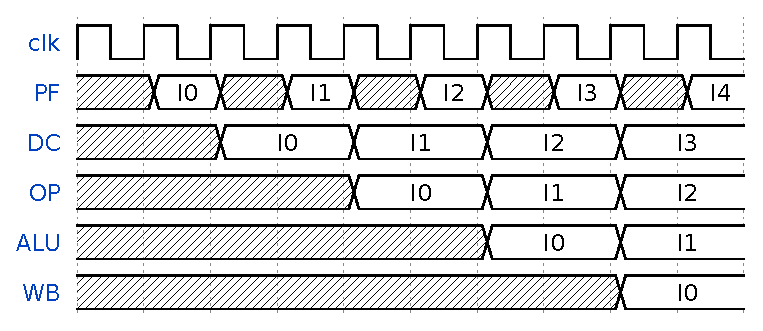
\includegraphics[width=4in]{../gfx/stuttra.eps}
\caption{Instructions wait for each other}\label{fig:waiting-pipeline}
\end{center}\end{figure}
	where instructions are held back until the pipeline is full, or should
	it look like Fig.~\ref{fig:independent-pipeline},
\begin{figure}\begin{center}
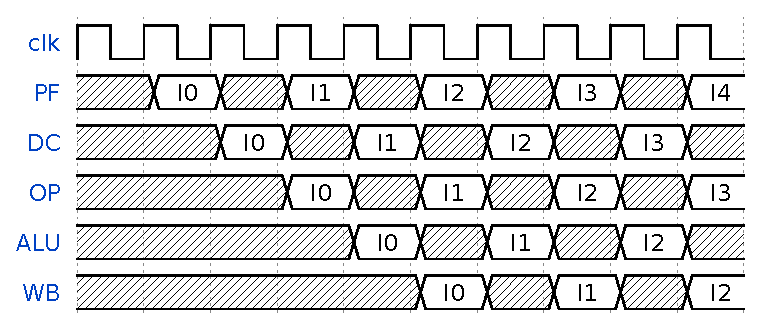
\includegraphics[width=4in]{../gfx/stuttrb.eps}
\caption{Instructions proceed independently}\label{fig:independent-pipeline}
\end{center}\end{figure}
	where each instruction is allowed to move through the pipeline
	independently?  For better or worse, the Zip CPU allows instructions
	to move through the pipeline independently.

	One approach to avoiding stalls is to use a branch delay slot,
	such as is shown in Fig.~\ref{fig:brdelay}.
\begin{figure}\begin{center}

\includegraphics[width=4in]{../gfx/bdly.eps}
\caption{A typical branch delay slot approach}\label{fig:brdelay}
\end{center}\end{figure}
	In this figure, instructions
	{\tt BR} (a branch), {\tt BD} (a branch delay instruction),
	are followed by instructions after the branch: {\tt IA}, {\tt IB}, etc.
	Since it takes a processor a clock cycle to execute a branch, the
	delay slot allows the processor to do something useful in that
	branch.  The problem the Zip CPU has with this approach is, what
	happens when the pipeline looks like Fig.~\ref{fig:brbroken}?
\begin{figure}\begin{center}
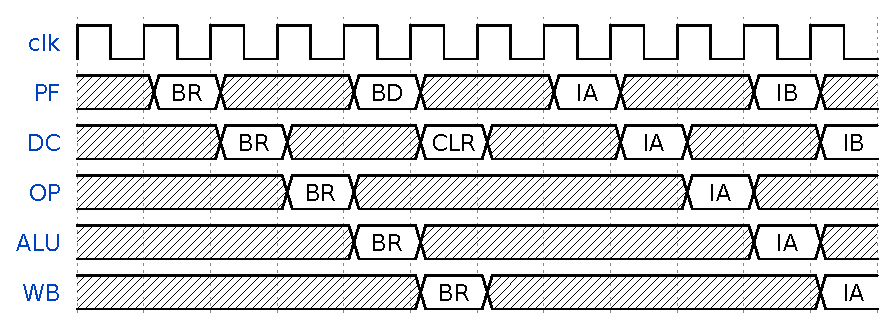
\includegraphics[width=4in]{../gfx/bdbroken.eps}
\caption{The branch delay slot breaks with a slow memory}\label{fig:brbroken}
\end{center}\end{figure}
	In this case, the branch delay slot never gets filled in the first
	place, and so the pipeline squashes it before it gets executed.
	If not that, then what happens when handling interrupts or
	debug stepping: when has the CPU finished an instruction?
	When the {\tt BR} instruction has finished, or must {\tt BD}
	follow every {\tt BR}?  and, again, what if the pipeline isn't
	full?
	These thoughts killed any hopes of doing delayed branching.

	So I switched to a model of discrete execution: Once an instruction
	enters into either the ALU or memory unit, the instruction is
	guaranteed to complete.  If the logic recognizes a branch or a 
	condition that would render the instruction entering into this stage
	possibly inappropriate (i.e. a conditional branch preceding a store
	instruction for example), then the pipeline stalls for one cycle
	until the conditional branch completes.  Then, if it generates a new
	PC address, the stages preceding are all wiped clean.

	This model, however, generated too many pipeline stalls, so the
	discrete execution model was modified to allow instructions to go
	through the ALU unit and be canceled before writeback.  This removed
	the stall associated with ALU instructions before untaken branches.

	The discrete execution model allows such things as sleeping, as
	outlined in Fig.~\ref{fig:sleeping}. 
\begin{figure}\begin{center}
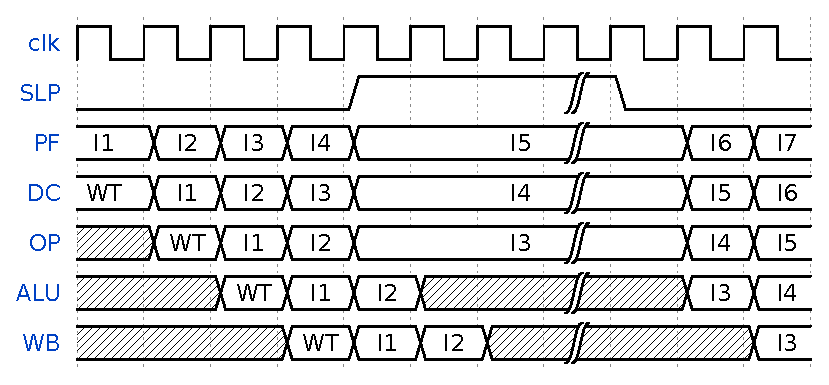
\includegraphics[width=4in]{../gfx/sleep.eps}
\caption{How the CPU halts when sleeping}\label{fig:sleeping}
\end{center}\end{figure}
	If the
	CPU is put to ``sleep,'' the ALU and memory stages stall and back up
	everything before them.  Likewise, anything that has entered the ALU
	or memory stage when the CPU is placed to sleep continues to completion.	
	To handle this logic, each pipeline stage has three control signals:
	a valid signal, a stall signal, and a clock enable signal.  In
	general, a stage stalls if it's contents are valid and the next step
	is stalled.  This allows the pipeline to fill any time a later stage
	stalls, as illustrated in Fig.~\ref{fig:stacking}.
\begin{figure}\begin{center}
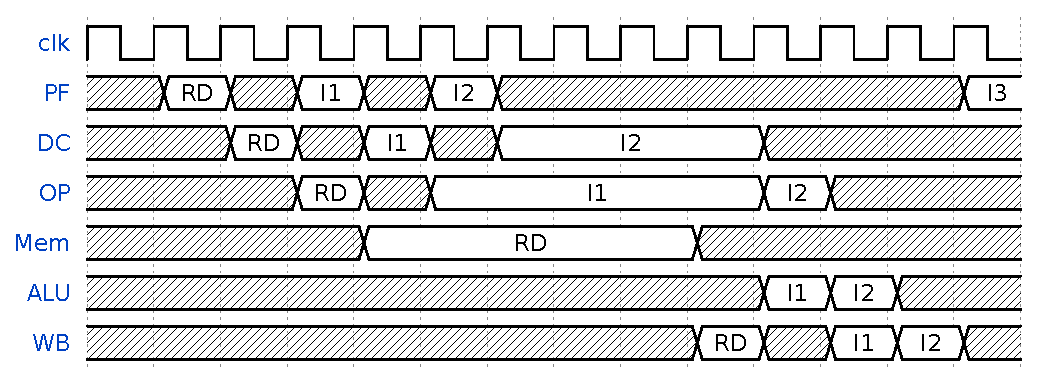
\includegraphics[width=4in]{../gfx/stacking.eps}
\caption{Instructions can stack up behind a stalled instruction}\label{fig:stacking}
\end{center}\end{figure}
	However, if a pipeline hazard is detected, a stage can stall in order
	to prevent the previous from moving forward.

	This approach is also different from other pipeline approaches. 
	Instead of keeping the entire pipeline filled, each stage is treated
	independently.  Therefore, individual stages may move forward as long
	as the subsequent stage is available, regardless of whether the stage
	behind it is filled.
\end{itemize}

With that introduction out of the way, let's move on to the instruction
set.

\chapter{CPU Architecture}\label{chap:arch}

The Zip CPU supports a set of two operand instructions, where the second operand
(always a register) is the result.  The only exception is the store instruction,
where the first operand (always a register) is the source of the data to be
stored.

\section{Simplified Bus}
The bus architecture of the Zip CPU is that of a simplified WISHBONE bus.
Several changes have been made to simplify this bus.  First, all unnecessary
ancillary information has been removed.  This includes the retry, tag, and
cycle type indicator signals.  Second, all operations on the bus are 32--bit
operations.  The bus is neither little endian nor big endian.  For this
reason, all words are 32--bits.  All instructions are also 32--bits wide. 
Everything has been built around the 32--bit word.  Even the byte size
(the size of the minimum addressable unit) is 32--bits.  This allows us to
remove the select lines from the wishbone bus.  Third, we insist that all
accesses be pipelined, and simplify that further by insisting that pipelined
accesses not cross peripherals---although we leave the user to keep that
from happening in practice.  Finally, we insist that the wishbone strobe line
be zero any time the cycle line is inactive.  This makes decoding simpler
in slave logic: a transaction is initiated whenever the strobe line is high
and the stall line is low.  The transaction completes whenever either the
ACK or the ERR lines go high.

\section{Register Set}
The Zip CPU supports two sets of sixteen 32-bit registers, a supervisor
and a user set as shown in Fig.~\ref{fig:regset}. 
\begin{figure}\begin{center}
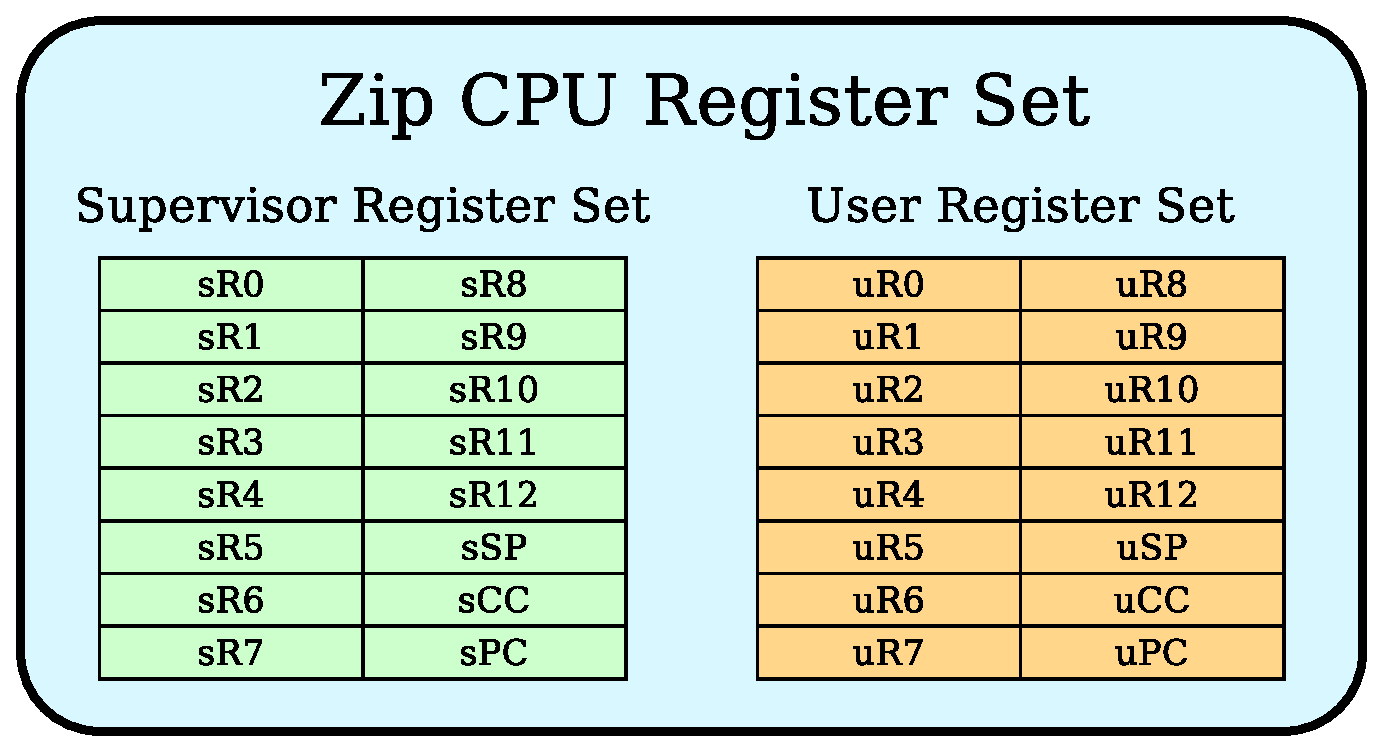
\includegraphics[width=3.5in]{../gfx/regset.eps}
\caption{Zip CPU Register File}\label{fig:regset}
\end{center}\end{figure}
The supervisor set is used in interrupt mode when interrupts are disabled,
whereas the user set is used any time interrupts are enabled.  Indeed, it is
impossible to enable interrupts without switching to the user instruction
set.  Of this register set, the Program Counter (PC) is register 15, whereas
the status register (SR) or condition code register (CC) is register 14.  All
other registers are identical in their hardware functionality---with the
exception that jumps to R0 (i.e., return from subroutines) may be optimized in
the future within the early branch logic.
By convention, the stack pointer will be register 13 and
noted as (SP)--although there is nothing special about this register other
than this convention.  Also by convention, if the compiler needs a frame pointer
it will be placed into register~12, and may be abbreviated by FP.  Finally,
by convention, R0 will hold a subroutines return address.
When the CPU is in supervisor mode, instructions can access both register sets
via move instruction, whereas when the CPU is in user mode, move instructions
will only offer access to user registers.

The status register (CC) is special, and bears further mention.  As shown in 
Fig.~\ref{tbl:cc-register},
\begin{table}\begin{center}
\begin{bitlist}
31\ldots 23 & R & Reserved for future uses\\\hline
22\ldots 16 & R/W & Reserved for future uses\\\hline
15 & R & Reserved for MMU exceptions\\\hline
14 & W & Clear I-Cache command, always reads zero\\\hline
13 & R & VLIW instruction phase (1 for first half)\\\hline
12 & R & (Reserved for) Floating Point Exception\\\hline
11 & R & Division by Zero Exception\\\hline
10 & R & Bus-Error Flag\\\hline
9 & R & Trap Flag (or user interrupt).  Cleared on return to userspace.\\\hline
8 & R & Illegal Instruction Flag\\\hline
7 & R/W & Break--Enable (sCC), or user break (uCC)\\\hline
6 & R/W & Step\\\hline
5 & R/W & Global Interrupt Enable (GIE)\\\hline
4 & R/W & Sleep.  When GIE is also set, the CPU waits for an interrupt.\\\hline
3 & R/W & Overflow\\\hline
2 & R/W & Negative.  The sign bit was set as a result of the last ALU instruction.\\\hline
1 & R/W & Carry\\\hline
0 & R/W & Zero.  The last ALU operation produced a zero.\\\hline
\end{bitlist}
\caption{Condition Code Register Bit Assignment}\label{tbl:cc-register}
\end{center}\end{table}
the lower 15~bits of the status register form
a set of CPU state and condition codes.  Writes to other bits of this register
are preserved.

Of the condition codes, the bottom four bits are the current flags:
		Zero (Z),
		Carry (C),
		Negative (N),
		and Overflow (V).
On those instructions that set the flags, these flags will be set based upon
the output of the instruction.  If the result is zero, the Z flag will be set.
If the high order bit is set, the N flag will be set.  If the instruction
caused a bit to fall off the end, the carry bit will be set.  In comparisons,
this is equivalent to a less--than unsigned comparison.  Finally, if
the instruction causes a signed integer overflow, the V flag will be set
afterwards.

The next bit is a sleep bit.  Set this bit to one to disable instruction
	execution and place the CPU to sleep, or to zero to keep the pipeline
	running.  Setting this bit will cause the CPU to wait for an interrupt
	(if interrupts are enabled), or to completely halt (if interrupts are
	disabled).  In order to prevent users from halting the CPU, only the
	supervisor is allowed to both put the CPU to sleep and disable
	interrupts.  Any user attempt to do so will simply result in a switch
	to supervisor mode.

The sixth bit is a global interrupt enable bit (GIE).  When this
	sixth bit is a `1' interrupts will be enabled, else disabled.  When 
	interrupts are disabled, the CPU will be in supervisor mode, otherwise
	it is in user mode.  Thus, to execute a context switch, one only
	need enable or disable interrupts.  (When an interrupt line goes
	high, interrupts will automatically be disabled, as the CPU goes
	and deals with its context switch.)  Special logic has been added to
	keep the user mode from setting the sleep register and clearing the
	GIE register at the same time, with clearing the GIE register taking
	precedence.

The seventh bit is a step bit.  This bit can be set from supervisor mode only.
	After setting this bit, should the supervisor mode process switch to
	user mode, it would then accomplish one instruction in user mode
	before returning to supervisor mode.  Then, upon return to supervisor
	mode, this bit will be automatically cleared.  This bit has no effect
	on the CPU while in supervisor mode.

	This functionality was added to enable a userspace debugger
	functionality on a user process, working through supervisor mode
	of course.


The eighth bit is a break enable bit.  When applied to the supervisor CC
register, this controls whether a break instruction in user mode will halt
the processor for an external debugger (break enabled), or whether the break
instruction will simply send send the CPU into interrupt mode.  Encountering
a break in supervisor mode will halt the CPU independent of the break enable
bit.  This bit can only be set within supervisor mode.  However, when applied
to the user CC register, from supervisor mode, this bit will indicate whether
or not the reason the CPU entered supervisor mode was from a break instruction
or not.  This break reason bit is automatically cleared upon any transition to
user mode, although it can also be cleared by the supervisor writing to the
user CC register.

% Should break enable be a supervisor mode bit, while the break enable bit
% in user mode is a break has taken place bit?
%

This functionality was added to enable an external debugger to
	set and manage breakpoints.

The ninth bit is an illegal instruction bit.  When the CPU
tries to execute either a non-existant instruction, or an instruction from
an address that produces a bus error, the CPU will (if implemented) switch
to supervisor mode while setting this bit.  The bit will automatically be
cleared upon any return to user mode.

The tenth bit is a trap bit.  It is set whenever the user requests a soft
interrupt, and cleared on any return to userspace command.  This allows the
supervisor, in supervisor mode, to determine whether it got to supervisor
mode from a trap, from an external interrupt or both.

The eleventh bit is a bus error flag.  If the user program encountered a bus
error, this bit will be set in the user CC register and the CPU will switch to
supervisor mode.  The bit may be cleared by the supervisor, otherwise it is
automatically cleared upon any return to user mode.  If the supervisor
encounters a bus error, this bit will be set in the supervisor CC register
and the CPU will halt.  In that case, either a CPU reset or a write to the
supervisor CC register will clear this register.

The twelth bit is a division by zero exception flag.  This operates in a fashion
similar to the bus error flag.  If the user attempts to use the divide
instruction with a zero denominator, the system will switch to supervisor mode
and set this bit in the user CC register.  The bit is automatically cleared
upon any return to user mode, although it can also be manually cleared by
the supervisor.  In a similar fashion, if the supervisor attempts to execute
a divide by zero, the CPU will halt and set the zero exception flag in the
supervisor's CC register.  This will automatically be cleared upon any CPU
reset, or it may be manually cleared by the external debugger writing to this
register.

The thirteenth bit will operate in a similar fashion to both the bus error
and division by zero flags, only it will be set upon a (yet to be determined)
floating point error.

Finally, the fourteenth bit references a clear cache bit.  The supervisor may
write a one to this bit in order to clear the CPU instruction cache.  The
bit always reads as a zero.

Last, but not least, the fifteenth bit is reserved for a page not found
memory exception.

Some of the upper bits have been temporarily assigned to indicate CPU
capabilities.  This is not a permanent feature, as these upper bits officially
remain reserved.

\section{Instruction Format}
All Zip CPU instructions fit in one of the formats shown in
Fig.~\ref{fig:iset-format}.
\begin{figure}\begin{center}
\begin{bytefield}[endianness=big]{32}
\bitheader{0-31}\\
\begin{leftwordgroup}{Standard}\bitbox{1}{0}\bitbox{4}{DR}
		\bitbox[lrt]{5}{OpCode}
		\bitbox[lrt]{3}{Cnd}
		\bitbox{1}{0}
		\bitbox{18}{18-bit Signed Immediate} \\
\bitbox{1}{0}\bitbox{4}{DR}
		\bitbox[lrb]{5}{}
		\bitbox[lrb]{3}{}
		\bitbox{1}{1}
		\bitbox{4}{BR}
		\bitbox{14}{14-bit Signed Immediate}\end{leftwordgroup} \\
\begin{leftwordgroup}{MOV}\bitbox{1}{0}\bitbox{4}{DR}
		\bitbox[lrt]{5}{5'hf}
		\bitbox[lrt]{3}{Cnd}
		\bitbox{1}{A}
		\bitbox{4}{BR}
		\bitbox{1}{B}
		\bitbox{13}{13-bit Signed Immediate}\end{leftwordgroup} \\
\begin{leftwordgroup}{LDI}\bitbox{1}{0}\bitbox{4}{DR}
		\bitbox{4}{4'hb}
		\bitbox{23}{23-bit Signed Immediate}\end{leftwordgroup} \\
\begin{leftwordgroup}{NOOP}\bitbox{1}{0}\bitbox{3}{3'h7}
		\bitbox{1}{}
		\bitbox{2}{11}
		\bitbox{3}{xxx}
		\bitbox{22}{Ignored}
		\end{leftwordgroup} \\
\begin{leftwordgroup}{VLIW}\bitbox{1}{1}\bitbox[lrt]{4}{DR}
		\bitbox[lrt]{5}{OpCode}
		\bitbox[lrt]{3}{Cnd}
		\bitbox{1}{0}
		\bitbox{4}{Imm.}
		\bitbox{14}{---} \\
\bitbox{1}{1}\bitbox[lr]{4}{}
		\bitbox[lrb]{5}{}
		\bitbox[lr]{3}{}
		\bitbox{1}{1}
		\bitbox{4}{BR}
		\bitbox{14}{---}	\\
\bitbox{1}{1}\bitbox[lrb]{4}{}
		\bitbox{4}{4'hb}
		\bitbox{1}{}
		\bitbox[lrb]{3}{}
		\bitbox{5}{5'b Imm}
		\bitbox{14}{---}	\\
\bitbox{1}{1}\bitbox{9}{---}
		\bitbox[lrt]{3}{Cnd}
		\bitbox{5}{---}
		\bitbox[lrt]{4}{DR}
		\bitbox[lrt]{5}{OpCode}
		\bitbox{1}{0}
		\bitbox{4}{Imm}
		\\
\bitbox{1}{1}\bitbox{9}{---}
		\bitbox[lr]{3}{}
		\bitbox{5}{---}
		\bitbox[lr]{4}{}
		\bitbox[lrb]{5}{}
		\bitbox{1}{1}
		\bitbox{4}{Reg} \\
\bitbox{1}{1}\bitbox{9}{---}
		\bitbox[lrb]{3}{}
		\bitbox{5}{---}
		\bitbox[lrb]{4}{}
		\bitbox{4}{4'hb}
		\bitbox{1}{}
		\bitbox{5}{5'b Imm}
		\end{leftwordgroup} \\
\end{bytefield}
\caption{Zip Instruction Set Format}\label{fig:iset-format}
\end{center}\end{figure}
The basic format is that some operation, defined by the OpCode, is applied
if a condition, Cnd, is true in order to produce a result which is placed in
the destination register, or DR.  The load 23--bit signed immediate instruction
(LDI) is different in that it accepts no conditions, and uses only a 4-bit
opcode.

This is actually a second version of instruction set definition, given certain
lessons learned.  For example, the original instruction set had the following
problems:
\begin{enumerate}
\item No opcodes were available for divide or floating point extensions to be
	made available.  Although there was space in the instruction set to
	add these types of instructions, this instruction space was going to
	require extra logic to use.
\item The carveouts for instructions such as NOOP and LDILO required
	extra logic to process.
\item The instruction set wasn't very compact.  One bus operation was required
	for every instruction.
\item While the CPU supported multiplies, they were only 16x16 bit multiplies.
\end{enumerate}
This second version was designed with two criteria.  The first was that the
new instruction set needed to be compatible, at the assembly language level,
with the previous instruction set.  Thus, it must be able to support all of
the previous mneumonics and more.  This was achieved with the sole exception
that instruction immediates are generally two bits shorter than before.
(One bit was lost to the VLIW bit in front, another from changing from 4--bit
to 5--bit opcodes.)  Second, the new instruction set needed to be a drop--in
replacement for the decoder, modifying nothing else.  This was almost achieved,
save for two issues: the ALU unit needed to be replaced since the OpCodes
were reordered, and some condition code logic needed to be adjusted since the
condition codes were renumbered as well.  In the end, maximum reuse of the
existing RTL (Verilog) code was achieved in this upgrade.

As of this second version of the Zip CPU instruction set, the Zip CPU also
supports a very long instruction word (VLIW) set of instructions.   These
instruction formats pack two instructions into a single instuction word,
trading immediate instruction space to do this, but in just about all other
respects these are identical to two standard instructions.  Other than 
instruction format, the only basic difference is that the CPU will not switch
to interrupt mode in between the two instructions.  Likewise a new job given
to the assembler is that of automatically packing as many instructions as
possible into the VLIW format.  Where necessary to place both VLIW instructions
on the same line, they will be separated by a vertical bar.

One belated change to the instruction set violates some of the above
principles.  This latter instruction set change replaced the {\tt LDIHI}
instruction with a 32--bit multiply instruction {\tt MPY}, and then changed
the two 16--bit multiply instructions {\tt MPYU} and {\tt MPYS} for 
{\tt MPYUHI} and {\tt MPYSHI} respectively.  This creates a 32--bit 
multiply capability, while removing the 16--bit multiply that wasn't very
useful. Further, the {\tt LDIHI} instruction was being used primarily by the
assembler and linker to create a 32--bit load immediate pair of instructions.
This instruction set combination, {\tt LDIHI} followed by {\tt LDILO} was
replaced with an equivalent instruction set, {\tt BREV} followed by {\tt LDILO},
save that linking has been made more complicated in the process since the
{\tt BREV} requires that the immediate be bit--reversed.

\section{Instruction OpCodes}
With a 5--bit opcode field, there are 32--possible instructions as shown in 
Tbl.~\ref{tbl:iset-opcodes}.
\begin{table}\begin{center}
\begin{tabular}{|l|l|l|c|} \hline \rowcolor[gray]{0.85}
OpCode & & Instruction &Sets CC \\\hline\hline
5'h00 & SUB & Subtract &   \\\cline{1-3}
5'h01 & AND & Bitwise And &   \\\cline{1-3}
5'h02 & ADD & Add two numbers &   \\\cline{1-3}
5'h03 & OR  & Bitwise Or & Y \\\cline{1-3}
5'h04 & XOR & Bitwise Exclusive Or &   \\\cline{1-3}
5'h05 & LSR & Logical Shift Right &   \\\cline{1-3}
5'h06 & LSL & Logical Shift Left &   \\\cline{1-3}
5'h07 & ASR & Arithmetic Shift Right &   \\\hline
5'h08 & MPY & 32x32 bit multiply & Y \\\hline
5'h09 & LDILO & Load Immediate Low & N\\\hline
5'h0a & MPYUHI & Upper 32 of 64 bits from an unsigned 32x32 multiply &  \\\cline{1-3}
5'h0b & MPYSHI & Upper 32 of 64 bits from a signed 32x32 multiply & Y \\\cline{1-3}
5'h0c & BREV & Bit Reverse B operand into result&  \\\cline{1-3}
5'h0d & POPC& Population Count &  \\\cline{1-3}
5'h0e & ROL & Rotate Ra left by OpB bits&   \\\hline
5'h0f & MOV & Move OpB into Ra & N \\\hline
5'h10 & CMP & Compare (Ra-OpB) to zero & Y \\\cline{1-3}
5'h11 & TST & Test (AND w/o setting result) &   \\\hline
5'h12 & LOD & Load Ra from memory (OpB) & N \\\cline{1-3}
5'h13 & STO & Store Ra into memory at (OpB) &  \\\hline\hline
5'h14 & DIVU & Divide, unsigned & Y \\\cline{1-3}
5'h15 & DIVS & Divide, signed &  \\\hline\hline
5'h16/7 & LDI & Load 23--bit signed immediate & N \\\hline\hline
5'h18 & FPADD & Floating point add &  \\\cline{1-3}
5'h19 & FPSUB & Floating point subtract &   \\\cline{1-3}
5'h1a & FPMPY & Floating point multiply & Y \\\cline{1-3}
5'h1b & FPDIV & Floating point divide &   \\\cline{1-3}
5'h1c & FPCVT & Convert integer to floating point &   \\\cline{1-3}
5'h1d & FPINT & Convert to integer &   \\\hline
5'h1e & & {\em Reserved for future use} &\\\hline
5'h1f & & {\em Reserved for future use} &\\\hline
5'h18 & & NOOP (A-register = PC)&\\\cline{1-3}
5'h19 & & BREAK (A-register = PC)& N\\\cline{1-3}
5'h1a & & LOCK (A-register = PC)&\\\hline
\end{tabular}
\caption{Zip CPU OpCodes}\label{tbl:iset-opcodes}
\end{center}\end{table}
%
Of these opcodes, {\tt POPC} is experimental and may be
replaced later.  There is room for six more register-less instructions,
and two floating point instruction opcodes have been reserved for future use.

\section{Conditional Instructions}
Most, although not quite all, instructions may be conditionally executed.  
The 23--bit load immediate instruction, together with the {\tt NOOP}, 
{\tt BREAK}, and {\tt LOCK} instructions are the only exception to this rule.
ALl other instructions may be conditionally executed.

From the four condition code flags, eight conditions are defined for standard
instructions.  These are shown in Tbl.~\ref{tbl:conditions}.
\begin{table}\begin{center}
\begin{tabular}{l|l|l}
Code & Mneumonic & Condition \\\hline
3'h0 & None & Always execute the instruction \\
3'h1 & {\tt .LT} & Less than ('N' set) \\
3'h2 & {\tt .Z} & Only execute when 'Z' is set \\
3'h3 & {\tt .NZ} & Only execute when 'Z' is not set \\
3'h4 & {\tt .GT} & Greater than ('N' not set, 'Z' not set) \\
3'h5 & {\tt .GE} & Greater than or equal ('N' not set, 'Z' irrelevant) \\
3'h6 & {\tt .C} & Carry set (Also known as less-than unsigned) \\
3'h7 & {\tt .V} & Overflow set\\
\end{tabular}
\caption{Conditions for conditional operand execution}\label{tbl:conditions}
\end{center}\end{table}
There is no condition code for less than or equal, not C or not V---there
just wasn't enough space in 3--bits.  Conditioning on a non--supported
condition is still possible, but it will take an extra instruction and a
pipeline stall.  (Ex: \hbox{\em (Stall)}; \hbox{\tt TST \$4,CC;} \hbox{\tt
STO.NZ R0,(R1)}) As an alternative, it is often possible to reverse the
condition, and thus recovering those extra two clocks.  Thus instead of
\hbox{\tt CMP Rx,Ry;} \hbox{\tt BNC label} you can issue a
\hbox{\tt CMP 1+Ry,Rx;} \hbox{\tt BC label}.

Conditionally executed instructions will not further adjust the 
condition codes, with the exception of \hbox{\tt CMP} and \hbox{\tt TST}
instructions.   Conditional \hbox{\tt CMP} or \hbox{\tt TST} instructions
will adjust conditions whenever they are executed.  In this way,
multiple conditions may be evaluated without branches.  For example, to do
something if \hbox{\tt R0} is one and \hbox{\tt R1} is two, one might try
code such as Tbl.~\ref{tbl:dbl-condition}.
\begin{table}\begin{center}
\begin{tabular}{l}
	{\tt CMP 1,R0} \\
	{;\em Condition codes are now set based upon R0-1} \\
	{\tt CMP.Z 2,R1} \\
	{;\em If R0 $\neq$ 1, conditions are unchanged, {\tt Z} is still false.} \\
	{;\em If R0 $=$ 1, conditions are now set based upon R1-2.} \\
	{;\em Now some instruction could be done based upon the conjunction} \\
	{;\em of both conditions.} \\
	{;\em While we use the example of a STO, it could easily be any instruction.} \\
	{\tt STO.Z R0,(R2)} \\
\end{tabular}
\caption{An example of a double conditional}\label{tbl:dbl-condition}
\end{center}\end{table}

The real utility of conditionally executed instructions is that, unlike
conditional branches, conditionally executed instructions will not stall
the bus if they are not executed.

In the case of VLIW instructions, only four conditions are defined as shown 
in Tbl.~\ref{tbl:vliw-conditions}.
\begin{table}\begin{center}
\begin{tabular}{l|l|l}
Code & Mneumonic & Condition \\\hline
2'h0 & None & Always execute the instruction \\
2'h1 & {\tt .LT} & Less than ('N' set) \\
2'h2 & {\tt .Z} & Only execute when 'Z' is set \\
2'h3 & {\tt .NZ} & Only execute when 'Z' is not set \\
\end{tabular}
\caption{VLIW Conditions}\label{tbl:vliw-conditions}
\end{center}\end{table}
Further, the first bit is given a special meaning.  If the first bit is set,
the conditions apply to the second half of the instruction, otherwise the
conditions will only apply to the first half of a conditional instruction.
Of course, the other conditions are still available by mingling the
non--VLIW instructions with VLIW instructions.

\section{Operand B}
Many instruction forms have a 19-bit source ``Operand B'', or OpB for short,
associated with them.  This ``Operand B'' is shown in
Fig.~\ref{fig:iset-format} as part of the standard instructions.  An Operand B
is either equal to a register plus a 14--bit signed immediate offset, or an
18--bit signed immediate offset by itself.  This value is encoded as shown in
Tbl.~\ref{tbl:opb}.
\begin{table}\begin{center}
\begin{bytefield}[endianness=big]{19}
\bitheader{0-18}  \\
\bitbox{1}{0}\bitbox{18}{18-bit Signed Immediate} \\
\bitbox{1}{1}\bitbox{4}{Reg}\bitbox{14}{14-bit Signed Immediate}
\end{bytefield}
\caption{Bit allocation for Operand B}\label{tbl:opb}
\end{center}\end{table}

Fourteen and eighteen bit immediate values don't make sense for all
instructions.  For example, what is the point of an 18--bit immediate when
executing a 16--bit multiply?  Or a 16--bit load--immediate?  In these cases,
the extra bits are simply ignored.

VLIW instructions still use the same operand B, only there was no room for any
instruction plus immediate addressing.  Therefore, VLIW instructions have either
a register or a 4--bit signed immediate as their operand B.  The only exception
is the load immediate instruction, which permits a 5--bit signed operand
B.\footnote{Although the space exists to extend this VLIW load immediate
instruction to six bits, the 5--bit limit was chosen to simplify the
disassembler.  This may change in the future.}

\section{Address Modes}
The Zip CPU supports two addressing modes: register plus immediate, and
immediate address.  Addresses are therefore encoded in the same fashion as
Operand B's, shown above.  Practically, the VLIW instruction set only offers
register addressing, necessitating a non--VLIW instruction for most memory
operations.

A lot of long hard thought was put into whether to allow pre/post increment
and decrement addressing modes.  Finding no way to use these operators without
taking two or more clocks per instruction,\footnote{The two clocks figure
comes from the design of the register set, allowing only one write per clock.
That write is either from the memory unit or the ALU, but never both.} these
addressing modes have been
removed from the realm of possibilities.  This means that the Zip CPU has no
native way of executing push, pop, return, or jump to subroutine operations.
Each of these instructions can be emulated with a set of instructions from the
existing set.

\section{Modifying Conditions}
A quick look at the list of conditions supported by the Zip CPU and listed
in Tbl.~\ref{tbl:conditions} reveals that the Zip CPU does not have a full set
of conditions.  In particular, only one explicit unsigned condition is
supported.  Therefore, Tbl.~\ref{tbl:creating-conditions}
\begin{table}\begin{center}
\begin{tabular}{|l|l|l|}\hline
Original & Modified & Name \\\hline\hline
\parbox[t]{1.5in}{\tt CMP Rx,Ry\\BLE label} % If Ry <= Rx -> Ry < Rx+1
	& \parbox[t]{1.5in}{\tt CMP 1+Rx,Ry\\BLT label}
	& Less-than or equal (signed, {\tt Z} or {\tt N} set)\\[4mm]\hline
\parbox[t]{1.5in}{\tt CMP Rx,Ry\\BLEU label}
	& \parbox[t]{1.5in}{\tt CMP 1+Rx,Ry\\BC label}
	& Less-than or equal unsigned \\[4mm]\hline
\parbox[t]{1.5in}{\tt CMP Rx,Ry\\BGTU label}	% if (Ry > Rx) -> Rx < Ry
	& \parbox[t]{1.5in}{\tt CMP Ry,Rx\\BC label}
	& Greater-than unsigned \\[4mm]\hline
\parbox[t]{1.5in}{\tt CMP Rx,Ry\\BGEU label}	% if (Ry >= Rx) -> Rx <= Ry -> Rx < Ry+1
	& \parbox[t]{1.5in}{\tt CMP 1+Ry,Rx\\BC label}
	& Greater-than equal unsigned \\[4mm]\hline
\parbox[t]{1.5in}{\tt CMP A+Rx,Ry\\BGEU label} % if (Ry >= A+Rx)-> A+Rx <= Ry -> Rx < Ry+1-A
	& \parbox[t]{1.5in}{\tt CMP (1-A)+Ry,Rx\\BC label}
	& Greater-than equal unsigned (with offset)\\[4mm]\hline
\parbox[t]{1.5in}{\tt CMP A,Ry\\BGEU label} % if (Ry >= A+Rx)-> A+Rx <= Ry -> Rx < Ry+1-A
	& \parbox[t]{1.5in}{\tt LDI (A-1),Rx\\CMP Ry,Rx\\BC label}
	& Greater-than equal comparison with a constant\\[4mm]\hline
\end{tabular}
\caption{Modifying conditions}\label{tbl:creating-conditions}
\end{center}\end{table}
shows examples of how these unsupported conditions can be created
simply by adjusting the compare instruction, for no extra cost in clocks.
Of course, if the compare originally had an immediate within it, that immediate
would need to be loaded into a register in order to do make some of these
adjustments.  This case is shown as the last case above.

\section{Move Operands}
The previous set of operands would be perfect and complete, save only that
the CPU needs access to non--supervisory registers while in supervisory mode. 
Therefore, the MOV instruction is special and offers access to these registers
\ldots when in supervisory mode.  To keep the compiler simple, the extra bits
are ignored in non-supervisory mode (as though they didn't exist), rather than
being mapped to new instructions or additional capabilities.  The bits
indicating which register set each register lies within are the A-User, marked
`A' in Fig.~\ref{fig:iset-format}, and B-User bits, marked as `B'.  When set
to a one, these refer to a user mode register.  When set to a zero, these
refer to a register in the current mode, whether user or supervisor.  Further,
because a load immediate instruction exists, there is no move capability
between an immediate and a register: all moves come from either a register or
a register plus an offset.

This actually leads to a bit of a problem: since the {\tt MOV} instruction
encodes which register set each register is coming from or moving to, how shall
a compiler or assembler know how to compile a MOV instruction without knowing
the mode of the CPU at the time?  For this reason, the compiler will assume
all MOV registers are supervisor registers, and display them as normal. 
Anything with the user bit set will be treated as a user register and displayed
special.  Since the CPU quietly ignores the supervisor bits while in user mode,
anything marked as a user register will always specify the user mode register.

\section{Multiply Operations}

The ZipCPU supports three separate 32x32-bit multiply
instructions: {\tt MPY}, {\tt MPYUHI}, and {\tt MPYSHI}.  The first of these
produces the low 32-bits of a 32x32-bit multiply result.  The second two
produce the upper 32-bits.  The first, {\tt MPYUHI}, produces the upper 32-bits
assuming the multiply was unsigned, whereas {\tt MPYSHI} assumes it was signed.
Each multiply instruction is independent of each other in execution, although
the compiler may use them quite dependently.

In an effort to maintain single clock pipeline timing, all three of these
multiplies have been slowed down in logic.  Thus, depending upon the setting
of {\tt OPT\_MULTIPLY} within {\tt cpudefs.v}, the multiply instructions
will either 1)~cause an ILLEGAL instruction error ({\tt OPT\_MULTIPLY=0}, or
no multiply support), 2)~take one additional clock ({\tt OPT\_MULTIPLY=1}),
or 3)~take two additional clocks ({\tt OPT\_MULTIPLY=2}). 

\section{Divide Unit}
The Zip CPU also has an optionial divide unit which can be built alongside the
ALU.  This divide unit provides the Zip CPU with another two instructions that
cannot be executed in a single cycle: {\tt DIVS}, or signed divide, and
{\tt DIVU}, the unsigned divide.  These are both 32--bit divide instructions,
dividing one 32--bit number by another.  In this case, the Operand B field,
whether it be register or register plus immediate, constitutes the denominator,
whereas the numerator is given by the other register.

The Divide is also a multi--clock instruction.  While the divide is running,
the ALU, any memory loads, and the floating point unit (if installed) will be
idle.  Once the divide completes, other units may continue.

Of course, divides can have errors: division by zero.  In the case of division
by zero, an exception will be caused that will send the CPU either from 
user mode to supervisor mode, or halt the CPU if it is already in supervisor
mode.  Upon the exception, the divide by zero bit will be set in the CC
register.  In the case of a user mode divide by zero, this will be cleared
by any return to user mode command.  The supervisor bit may be cleared upon
restart, or by the external debugger.

\section{NOOP, BREAK, and Bus Lock Instruction}
Three instructions within the opcode list in Tbl.~\ref{tbl:iset-opcodes}, are
somewhat special.  These are the {\tt NOOP}, {\tt Break}, and bus {\tt LOCK}
instructions.  These are encoded according to
Fig.~\ref{fig:iset-noop}, and have the following meanings:
\begin{figure}\begin{center}
\begin{bytefield}[endianness=big]{32}
\bitheader{0-31}\\
\begin{leftwordgroup}{NOOP}
\bitbox{1}{0}\bitbox{3}{3'h7}\bitbox{1}{}
	\bitbox{2}{11}\bitbox{3}{000}\bitbox{22}{Reserved for Simulator} \\
\bitbox{1}{1}\bitbox{3}{3'h7}\bitbox{1}{}
	\bitbox{2}{11}\bitbox{3}{000}\bitbox{22}{---} \\
\bitbox{1}{1}\bitbox{9}{---}\bitbox{3}{---}\bitbox{5}{---}
	\bitbox{3}{3'h7}\bitbox{1}{}\bitbox{2}{11}\bitbox{3}{001}
	\bitbox{5}{Rsrvd}
		\end{leftwordgroup} \\
\begin{leftwordgroup}{BREAK}
\bitbox{1}{0}\bitbox{3}{3'h7}
		\bitbox{1}{}\bitbox{2}{11}\bitbox{3}{001}\bitbox{22}{Reserved for debugger}
		\end{leftwordgroup} \\
\begin{leftwordgroup}{LOCK}
\bitbox{1}{0}\bitbox{3}{3'h7}
		\bitbox{1}{}\bitbox{2}{11}\bitbox{3}{010}\bitbox{22}{Ignored}
		\end{leftwordgroup} \\
\end{bytefield}
\caption{NOOP/Break/LOCK Instruction Format}\label{fig:iset-noop}
\end{center}\end{figure}

The {\tt NOOP} instruction is just that: an instruction that does not perform
any operation.  While many other instructions, such as a move from a register
to itself, could also fit these roles, only the NOOP instruction guarantees
that it will not stall waiting for a register to be available.   For this
reason, it gets its own place in the instruction set.  Bits 21--0 of this
instruction are reserved for commands which may be given to a simulator, such
as simulator exit, should the code be run from a simulator.  However, such
simulation codes have not yet been defined.

The {\tt BREAK} instruction is useful for creating a debug instruction that
will halt the CPU without executing.  If in user mode, depending upon the
setting of the break enable bit, it will either switch to supervisor mode or
halt the CPU--depending upon where the user wishes to do his debugging.  The
lower 22~bits of this instruction are likewise reserved for the debuggers
use.

Finally, the {\tt LOCK} instruction was added in order to provide for
atomic operations.  The {\tt LOCK} instruction only works when the CPU was
compiled for in pipeline mode.  It works by stalling the ALU pipeline stack
until all prior stages are filled, and then it guarantees that once a bus
cycle is started, the wishbone {\tt CYC} line will remain asserted until the
LOCK is deasserted.  This allows the execution of one instruction that was
waiting in the load operands pipeline stage, and one instruction that was
waiting in the instruction decode stage.  Further, if the instruction waiting
in the decode stage was a VLIW instruction, then it may be possible to execute
a third instruction.

This was originally written to implement an atomic test and set instruction,
such as a {\tt LOCK} followed by {\tt LOD (Rx),Ry} and a {\tt STO Rz,(Rx)},
where Rz is initially set.

Other instructions using a VLIW instruction combining a single ALU instruction
with a store, such as an atomic increment, or {\tt LOCK}, {\tt LOD (Rx),Ry},
{\tt ADD 1,Ry}, {\tt STO Ry,(Rx)}, should be possible as well.  Many of these
combinations remain to be tested.

\section{Floating Point}
Although the Zip CPU does not (yet) have a floating point unit, the current
instruction set offers eight opcodes for floating point operations, and treats
floating point exceptions like divide by zero errors.  Once this unit is built
and integrated together with the rest of the CPU, the Zip CPU will support
32--bit floating point instructions natively.  Any 64--bit floating point
instructions will either need to be emulated in software, or else they will
need an external floating point peripheral.

Until the FPU is built and integrated, of even afterwards if the floating point
unit is not installed by option, floating point instructions will trigger an
illegal instruction exception, which may be trapped and then implemented in
software.

\section{Derived Instructions}
The Zip CPU supports many other common instructions, but not all of them
are single cycle instructions.  The derived instruction tables,
Tbls.~\ref{tbl:derived-1}, \ref{tbl:derived-2}, \ref{tbl:derived-3} 
and~\ref{tbl:derived-4},
help to capture some of how these other instructions may be implemented on
the Zip CPU.  Many of these instructions will have assembly equivalents,
such as the branch instructions, to facilitate working with the CPU.
\begin{table}\begin{center}
\begin{tabular}{p{1.4in}p{1.5in}p{3in}}\\\hline
Mapped & Actual  & Notes \\\hline
{\tt ABS Rx}
	& \parbox[t]{1.5in}{\tt TST -1,Rx\\NEG.LT Rx}
	& Absolute value, depends upon derived NEG.\\\hline
\parbox[t]{1.4in}{\tt ADD Ra,Rx\\ADDC Rb,Ry}
	& \parbox[t]{1.5in}{\tt Add Ra,Rx\\ADD.C \$1,Ry\\Add Rb,Ry}
	& Add with carry \\\hline
{\tt BRA.Cond +/-\$Addr}
	& \hbox{\tt ADD.cond \$Addr+PC,PC}
	& Branch or jump on condition.  Works for 18--bit
		signed address offsets.\\\hline
% {\tt BRA.Cond +/-\$Addr}
% 	& \parbox[t]{1.5in}{\tt LDI \$Addr,Rx \\ ADD.cond Rx,PC}
% 	& Branch/jump on condition.  Works for 23 bit address offsets, but
% 	costs a register and an extra instruction.  With LDIHI and LDILO
% 	this can be made to work anywhere in the 32-bit address space, but yet
% 	cost an additional instruction still. \\\hline
% {\tt BNC PC+\$Addr}
%	& \parbox[t]{1.5in}{\tt Test \$Carry,CC \\ ADD.Z PC+\$Addr,PC}
%	& Example of a branch on an unsupported
%		condition, in this case a branch on not carry \\\hline
{\tt BUSY } & {\tt ADD \$-1,PC} & Execute an infinite loop \\\hline
{\tt CLRF.NZ Rx }
	& {\tt XOR.NZ Rx,Rx}
	& Clear Rx, and flags, if the Z-bit is not set \\\hline
{\tt CLR Rx }
	& {\tt LDI \$0,Rx}
	& Clears Rx, leaves flags untouched.  This instruction cannot be
		conditional. \\\hline
{\tt CLR.NZ Rx }
	& {\tt BREV \$0,Rx}
	& Clears Rx, leaves flags untouched.  This instruction can be executed
		conditionally. \\\hline
{\tt EXCH.W Rx }
	& {\tt ROL \$16,Rx}
	& Exchanges the top and bottom 16'bit words of Rx \\\hline
{\tt HALT }
	& {\tt Or \$SLEEP,CC}
	& This only works when issued in interrupt/supervisor mode.  In user
	mode this is simply a wait until interrupt instruction. \\\hline
{\tt INT } & {\tt LDI \$0,CC} & This is also known as a trap instruction\\\hline
{\tt IRET}
	& {\tt OR \$GIE,CC}
	& Also known as an RTU instruction (Return to Userspace) \\\hline
{\tt JMP R6+\$Offset}
	& {\tt MOV \$Offset(R6),PC}
	& Only works for 13--bit offsets.\\\hline
{\tt LJMP \$Addr}
	& \parbox[t]{1.5in}{\tt LOD (PC),PC \\ {\em Address }}
	& Although this only works for an unconditional jump, and it only
	works in a Von Neumann architecture, this instruction combination makes
	for a nice combination that can be adjusted by a linker at a later
	time.\\\hline
{\tt LJMP.x \$Addr}
	& \parbox[t]{1.5in}{\tt LOD.x 2(PC),PC \\ ADD 1,PC \\ {\em Address }}
	& Long jump, works for a conditional long jump \\\hline
{\tt LJSR \$Addr  }
	& \parbox[t]{1.5in}{\tt MOV \$2+PC,R0 \\ LOD (PC),PC \\ {\em Address}}
	& Similar to LJMP, but it handles the return address properly.
	\\\hline
{\tt JSR PC+\$Offset  }
	& \parbox[t]{1.5in}{\tt MOV \$1+PC,R0 \\ ADD \$Offset,PC}
	& This is similar to the jump and link instructions from other
	architectures, save only that it requires a specific link
	instruction, also known as the {\tt MOV} instruction on the
	left.\\\hline
\end{tabular}
\caption{Derived Instructions}\label{tbl:derived-1}
\end{center}\end{table}
\begin{table}\begin{center}
\begin{tabular}{p{1.4in}p{1.5in}p{3in}}\\\hline
Mapped & Actual  & Notes \\\hline
{\tt LDI \$val,Rx }
	& \parbox[t]{1.8in}{\tt BERV REV($val$)\&0x0ffff), Rx \\
			LDILO (\$val\&0x0ffff),Rx}
	& \parbox[t]{3.0in}{Sadly, there's not enough instruction
		space to load a complete immediate value into any register.
		Therefore, fully loading any register takes two cycles.
		The {\tt LDILO} (load immediate low) instruction has been
		created to facilitate this together with {\tt BREV}.
		\\
	This is also the appropriate means for setting a register value
	to an arbitrary 32--bit value in a post--assembly link
	operation.}\\\hline
{\tt LOD.b \$addr,Rx}
	& \parbox[t]{1.5in}{\tt %
	LDI	\$addr,Ra \\
	LDI	\$addr,Rb \\
	LSR	\$2,Ra \\
	AND	\$3,Rb \\
	LOD	(Ra),Rx \\
	LSL	\$3,Rb \\
	SUB	\$32,Rb \\
	ROL	Rb,Rx \\
	AND \$0ffh,Rx}
	& \parbox[t]{3in}{This CPU is designed for 32'bit word
	length instructions.  Byte addressing is not supported by the CPU or
	the bus, so it therefore takes more work to do. 

	Note also that in this example, \$Addr is a byte-wise address, where
	all other addresses in this document are 32-bit wordlength addresses. 
	For this reason,
	we needed to drop the bottom two bits.  This also limits the address
	space of character accesses using this method from 16 MB down to 4MB.}
		\\\hline
\parbox[t]{1.5in}{\tt LSL \$1,Rx\\ LSLC \$1,Ry}
	& \parbox[t]{1.5in}{\tt LSL \$1,Ry \\
	LSL \$1,Rx \\
	OR.C \$1,Ry}
	& Logical shift left with carry.  Note that the
	instruction order is now backwards, to keep the conditions valid.
	That is, LSL sets the carry flag, so if we did this the other way
	with Rx before Ry, then the condition flag wouldn't have been right
	for an OR correction at the end. \\\hline
\parbox[t]{1.5in}{\tt LSR \$1,Rx \\ LSRC \$1,Ry}
	& \parbox[t]{1.5in}{\tt CLR Rz \\
	LSR \$1,Ry \\
	LDIHI.C \$8000h,Rz \\
	LSR \$1,Rx \\
	OR Rz,Rx}
	& Logical shift right with carry \\\hline
{\tt NEG Rx} & \parbox[t]{1.5in}{\tt XOR \$-1,Rx \\ ADD \$1,Rx} & \\\hline
{\tt NEG.C Rx} & \parbox[t]{1.5in}{\tt MOV.C \$-1+Rx,Rx\\XOR.C \$-1,Rx} & \\\hline
{\tt NOOP} & {\tt NOOP} & While there are many
	operations that do nothing, such as MOV Rx,Rx, or OR \$0,Rx, these
	operations have consequences in that they might stall the bus if
	Rx isn't ready yet.  For this reason, we have a dedicated NOOP
	instruction. \\\hline
{\tt NOT Rx } & {\tt XOR \$-1,Rx } & \\\hline
{\tt POP Rx }
	& \parbox[t]{1.5in}{\tt LOD \$(SP),Rx \\ ADD \$1,SP}
	& \\\hline
\end{tabular}
\caption{Derived Instructions, continued}\label{tbl:derived-2}
\end{center}\end{table}
\begin{table}\begin{center}
\begin{tabular}{p{1.4in}p{1.5in}p{3in}}\\\hline
{\tt PUSH Rx}
	& \parbox[t]{1.5in}{\hbox{\tt SUB \$1,SP} 
	\hbox{\tt STO Rx,\$(SP)}}
	& Note that for pipelined operation, it helps to coalesce all the
	{\tt SUB}'s into one command, and place the {\tt STO}'s right
	after each other.  Further, to avoid a pipeline stall, the
	immediate value for the first store must be zero.
	\\\hline
{\tt PUSH Rx-Ry}
	& \parbox[t]{1.5in}{\tt SUB \$$n$,SP \\
	STO Rx,\$(SP)
	\ldots \\
	STO Ry,\$$\left(n-1\right)$(SP)}
	& Multiple pushes at once only need the single subtract from the
	stack pointer.  This derived instruction is analogous to a similar one
	on the Motoroloa 68k architecture, although the Zip Assembler
	does not support the combined instruction.  This instruction
	also supports pipelined memory access.\\\hline
{\tt RESET}
	& \parbox[t]{1in}{\tt STO \$1,\$watchdog(R12)\\NOOP\\NOOP}
	& This depends upon the peripheral base address being
	preloaded into R12.

	Another opportunity might be to jump to the reset address from within
	supervisor mode.\\\hline
{\tt RET} & {\tt MOV R0,PC}
	& This depends upon the form of the {\tt JSR} given on the previous
	page that stores the return address into R0.
	\\\hline
{\tt STEP Rr,Rt}
	& \parbox[t]{1.5in}{\tt LSR \$1,Rr \\ XOR.C Rt,Rr}
	& Step a Galois implementation of a Linear Feedback Shift Register, Rr,
		using taps Rt \\\hline
%
%
{\tt SEX.b Rx }
	& \parbox[t]{1.5in}{\tt LSL 24,Rx \\ ASR 24,Rx}
	& Signed extend a byte into a full word.\\\hline
{\tt SEX.h Rx }	
	& \parbox[t]{1.5in}{\tt LSL 16,Rx \\ ASR 16,Rx}
	& Sign extend a half word into a full word.\\\hline
%
{\tt STO.b Rx,\$addr}
	& \parbox[t]{1.5in}{\tt %
	LDI \$addr,Ra \\
	LDI \$addr,Rb \\
	LSR \$2,Ra \\
	AND \$3,Rb \\
	SUB \$32,Rb \\
	LOD (Ra),Ry \\
	AND \$0ffh,Rx \\
	AND \~\$0ffh,Ry \\
	ROL Rb,Rx \\
	OR Rx,Ry \\
	STO Ry,(Ra) }
	& \parbox[t]{3in}{This CPU and it's bus are {\em not} optimized
	for byte-wise operations.
	
	Note that in this example, \$addr is a
	byte-wise address, whereas in all of our other examples it is a 
	32-bit word address. This also limits the address space
	of character accesses from 16 MB down to 4MB.F
	Further, this instruction implies a byte ordering,
	such as big or little endian.} \\\hline
{\tt SUBR Rx,Ry }
	& \parbox[t]{1.5in}{\tt SUB 1+Rx,Ry\\ XOR -1,Ry} 
	& Ry is set to Rx-Ry, rather than the normal subtract which
	sets Ry to Ry-Rx. \\\hline
\parbox[t]{1.4in}{\tt SUB Ra,Rx\\SUBC Rb,Ry}
	& \parbox[t]{1.5in}{\tt SUB Ra,Rx\\SUB.C \$1,Ry\\SUB Rb,Ry}
	& Subtract with carry \\\hline
\end{tabular}
\caption{Derived Instructions, continued}\label{tbl:derived-3}
\end{center}\end{table}
\begin{table}\begin{center}
\begin{tabular}{p{1.4in}p{1.5in}p{3in}}\\\hline
{\tt SWAP Rx,Ry }
	& \parbox[t]{1.5in}{\tt XOR Ry,Rx \\ XOR Rx,Ry \\ XOR Ry,Rx} 
	& While no extra registers are needed, this example
	does take 3-clocks. \\\hline
{\tt TRAP \#X}
	& \parbox[t]{1.5in}{\tt LDI \$x,R0 \\ AND \~\$GIE,CC }
	& This works because whenever a user lowers the \$GIE flag, it sets
	a TRAP bit within the CC register.  Therefore, upon entering the 
	supervisor state, the CPU only need check this bit to know that it
	got there via a TRAP.  The trap could be made conditional by making
	the LDI and the AND conditional.  In that case, the assembler would
	quietly turn the LDI instruction into an LDILO and LDIHI pair,
	but the effect would be the same. \\\hline
{\tt TS Rx,Ry,(Rz)}
	& \hbox{\tt LDI 1,Rx}
		\hbox{\tt LOCK}
		\hbox{\tt LOD (Rz),Ry}
		\hbox{\tt STO Rx,(Rz)}
	& A test and set instruction.  The {\tt LOCK} instruction insures
	that the next two instructions lock the bus between the instructions,
	so no one else can use it.  Thus guarantees that the operation is
	atomic.
	\\\hline
{\tt TST Rx}
	& {\tt TST \$-1,Rx}
	& Set the condition codes based upon Rx.  Could also do a CMP \$0,Rx,
	ADD \$0,Rx, SUB \$0,Rx, etc, AND \$-1,Rx, etc.  The TST and CMP 
	approaches won't stall future pipeline stages looking for the value
	of Rx. (Future versions of the assembler may shorten this to a 
	{\tt TST Rx} instruction.)\\\hline
{\tt WAIT}
	& {\tt Or \$GIE | \$SLEEP,CC}
	& Wait until the next interrupt, then jump to supervisor/interrupt
	mode.
\end{tabular}
\caption{Derived Instructions, continued}\label{tbl:derived-4}
\end{center}\end{table}

\section{Interrupt Handling}
The Zip CPU does not maintain any interrupt vector tables.  If an interrupt
takes place, the CPU simply switches to interrupt mode.  The supervisor code
continues in this interrupt mode from where it left off before, after 
executing a return to userspace {\tt RTU} instruction.

At this point, the supervisor code needs to determine first whether an 
interrupt has occurred, and then whether it is in interrupt mode due to 
an exception and handle each case appropriately.

\section{Pipeline Stages}
As mentioned in the introduction, and highlighted in Fig.~\ref{fig:cpu},
the Zip CPU supports a five stage pipeline.
\begin{enumerate}
\item {\bf Prefetch}: Reads instructions from memory and into a cache, if so 
	configured.  This
	stage is actually pipelined itself, and so it will stall if the PC
	ever changes.  Stalls are also created here if the instruction isn't
	in the prefetch cache.

	The Zip CPU supports one of three prefetch methods, depending upon a
	flag set at build time within the {\tt cpudefs.v} file.  The simplest
	is a non--cached implementation of a prefetch.  This implementation is
	fairly small, and ideal for users of the Zip CPU who need the extra
	space on the FPGA fabric.  However, because this non--cached version
	has no cache, the maximum number of instructions per clock is limited
	to about one per eight.

	The second prefetch module is a pipelined prefetch with a cache.  This
	module tries to keep the instruction address within a window of valid
	instruction addresses.  While effective, it is not a traditional
	cache implementation.  A disappointing feature of this implementation
	is that it needs an extra internal pipeline stage to be implemented.

	The third prefetch and cache module implements a more traditional
	cache.  This cache provides for the fastest CPU speed.  The only
	drawback is that, when a cache line is loading, the CPU cannot
	execute instructions from that cache line.

\item {\bf Decode}: Decodes an instruction into OpCode, register(s) to read,
	and immediate offset.  This stage also determines whether the flags
	will be set or whether the result will be written back.

\item {\bf Read Operands}: Read registers and apply any immediate values to
	them.  There is no means of detecting or flagging arithmetic overflow
	or carry when adding the immediate to the operand.  This stage will
	stall if any source operand is pending.

\item Split into one of four tracks: An {\bf ALU} track which will accomplish
	a simple instruction, the {\bf MemOps} stage which handles {\tt LOD}
	(load) and {\tt STO} (store) instructions, the {\bf divide} unit,
	and the {\bf floating point} unit.
	\begin{itemize}
	\item Loads will stall instructions in the decode stage until the
		entire pipeline until complete, lest a register be read in
		the read operands stage only to be updated unseen by the
		Load.
	\item Condition codes are available upon completion of the ALU,
		divide, or FPU stage.
	\item Issuing a non--pipelined memory instruction to the memory unit
		while the memory unit is busy will stall the entire pipeline. 
	\end{itemize}
\item {\bf Write-Back}: Conditionally write back the result to the register
	set, applying the condition.  This routine is quad-entrant: either the
	ALU, the memory, the divide, or the FPU may write back a register.
	The only design rule is that no more than a single register may be
	written back in any given clock.
\end{enumerate}

The Zip CPU does not support out of order execution.  Therefore, if the memory
unit stalls, every other instruction stalls.  The same is true for divide or
floating point instructions--all other instructions will stall while waiting
for these to complete.  Memory stores, however, can take place concurrently
with non--memory operations, although memory reads (loads) cannot.

\section{Pipeline Stalls}
The processing pipeline can and will stall for a variety of reasons.  Some of
these are obvious, some less so.  These reasons are listed below:
\begin{itemize}
\item When the prefetch cache is exhausted

This reason should be obvious.  If the prefetch cache doesn't have the
instruction in memory, the entire pipeline must stall until an instruction
can be made ready.  In the case of the {\tt pipefetch} windowed approach
to the prefetch cache, this means the pipeline will stall until enough of the
prefetch cache is loaded to support the next instruction.  In the case
of the more traditional {\tt pfcache} approach, the entire cache line must
fill before instruction execution can continue.

\item While waiting for the pipeline to load following any taken branch, jump,
	return from interrupt or switch to interrupt context (4 stall cycles)

Fig.~\ref{fig:bcstalls}
\begin{figure}\begin{center}
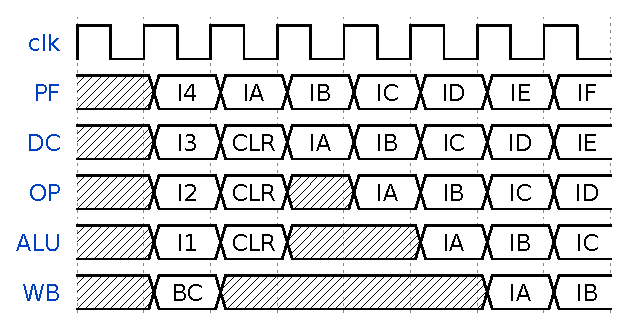
\includegraphics[width=3.5in]{../gfx/bc.eps}
\caption{A conditional branch generates 4 stall cycles}\label{fig:bcstalls}
\end{center}\end{figure}
illustrates the situation for a conditional branch.  In this case, the branch
instruction, {\tt BC}, is nominally followed by instructions {\tt I1} and so
forth.  However, since the branch is taken, the next instruction must be
{\tt IA}.  Therefore, the pipeline needs to be cleared and reloaded.
Given that there are five stages to the pipeline, that accounts
for the four stalls.  (Were the {\tt pipefetch} cache chosen, there would
be another stall internal to the {\tt pipefetch} cache.)

The Zip CPU handles the {\tt ADD \$X,PC} and
{\tt LDI \$X,PC} instructions specially, however.  These instructions, when
not conditioned on the flags, can execute with only a single stall cycle,
such as is shown in Fig.~\ref{fig:branch}.\footnote{Note that when using the
{\tt pipefetch} cache, this requires an additional stall cycle due to that
cache's implementation.}
\begin{figure}\begin{center}
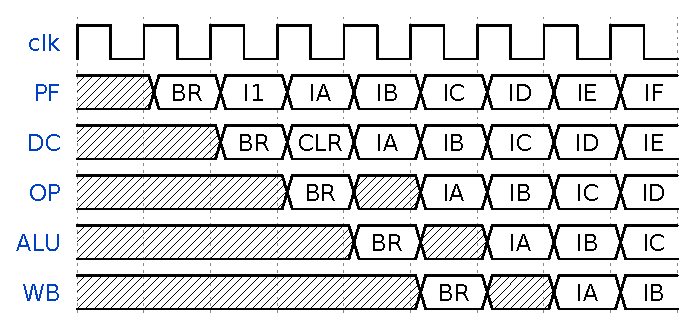
\includegraphics[width=4in]{../gfx/bra.eps} %0.4in per clock
\caption{An expedited branch costs a single stall cycle}\label{fig:branch}
\end{center}\end{figure}
In this example, {\tt BR} is a branch always taken, {\tt I1} is the instruction
following the branch in memory, while {\tt IA} is the first instruction at the
branch address.  ({\tt CLR} denotes a clear--pipeline operation, and does
not represent any instruction.)

\item When reading from a prior register while also adding an immediate offset
\begin{enumerate}
\item\ {\tt OPCODE ?,RA}
\item\ {\em (stall)}
\item\ {\tt OPCODE I+RA,RB}
\end{enumerate}

Since the addition of the immediate register within OpB decoding gets applied
during the read operand stage so that it can be nicely settled before the ALU,
any instruction that will write back an operand must be separated from the
opcode that will read and apply an immediate offset by one instruction.  The
good news is that this stall can easily be mitigated by proper scheduling.
That is, any instruction that does not add an immediate to {\tt RA} may be
scheduled into the stall slot.

This is also the reason why, when setting up a stack frame, the top of the
stack frame is used first: it eliminates this stall cycle.  Hence, to save
registers at the top of a procedure, one would write:
\begin{enumerate}
\item\ {\tt SUB 2,SP}
\item\ {\tt STO R1,(SP)}
\item\ {\tt STO R2,1(SP)}
\end{enumerate}
Had {\tt R1} instead been stored at {\tt 1(SP)} as the top of the stack,
there would've been an extra stall in setting up the stack frame.

\item When reading from the CC register after setting the flags
\begin{enumerate}
\item\ {\tt ALUOP RA,RB} {\em ; Ex: a compare opcode}
\item\ {\em (stall)}
\item\ {\tt TST sys.ccv,CC}
\item\ {\tt BZ somewhere}
\end{enumerate}

The reason for this stall is simply performance: many of the flags are
determined via combinatorial logic {\em during} the writeback cycle.
Trying to then place these into the input for one of the operands for an
ALU instruction during the same cycle
created a time delay loop that would no longer execute in a single 100~MHz
clock cycle.  (The time delay of the multiply within the ALU wasn't helping
either \ldots). 

This stall may be eliminated via proper scheduling, by placing an instruction
that does not set flags in between the ALU operation and the instruction
that references the CC register.  For example, {\tt MOV \$addr+PC,uPC}
followed by an {\tt RTU} ({\tt OR \$GIE,CC}) instruction will not incur
this stall, whereas an {\tt OR \$BREAKEN,CC} followed by an {\tt OR \$STEP,CC}
will incur the stall, while a {\tt LDI \$BREAKEN|\$STEP,CC} will not since
it doesn't read the condition codes before executing.

\item When waiting for a memory read operation to complete
\begin{enumerate}
\item\ {\tt LOD address,RA}
\item\ {\em (multiple stalls, bus dependent, 4 clocks best)}
\item\ {\tt OPCODE I+RA,RB}
\end{enumerate}

Remember, the Zip CPU does not support out of order execution.  Therefore,
anytime the memory unit becomes busy both the memory unit and the ALU must
stall until the memory unit is cleared.  This is illustrated in
Fig.~\ref{fig:memrd},
\begin{figure}\begin{center}
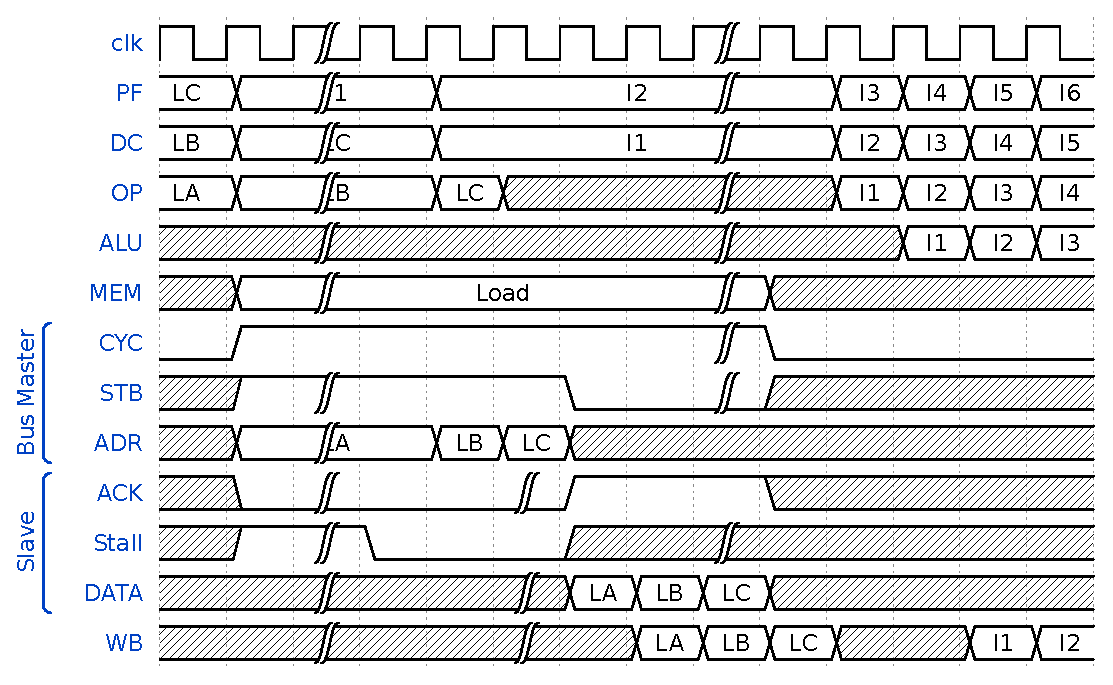
\includegraphics[width=5.6in]{../gfx/memrd.eps}
\caption{Pipeline handling of a load instruction}\label{fig:memrd}
\end{center}\end{figure}
since it is especially true of a load
instruction, which must still write its operand back to the register file.
Further, note that on a pipelined memory operation, the instruction must
stall in the decode operand stage, lest it try to read a result from the
register file before the load result has been written to it.  Finally, note
that there is an extra stall at the end of the memory cycle, so that
the memory unit will be idle for two clocks before an instruction will be
accepted into the ALU.  Store instructions are different, as shown in
Fig.~\ref{fig:memwr},
\begin{figure}\begin{center}
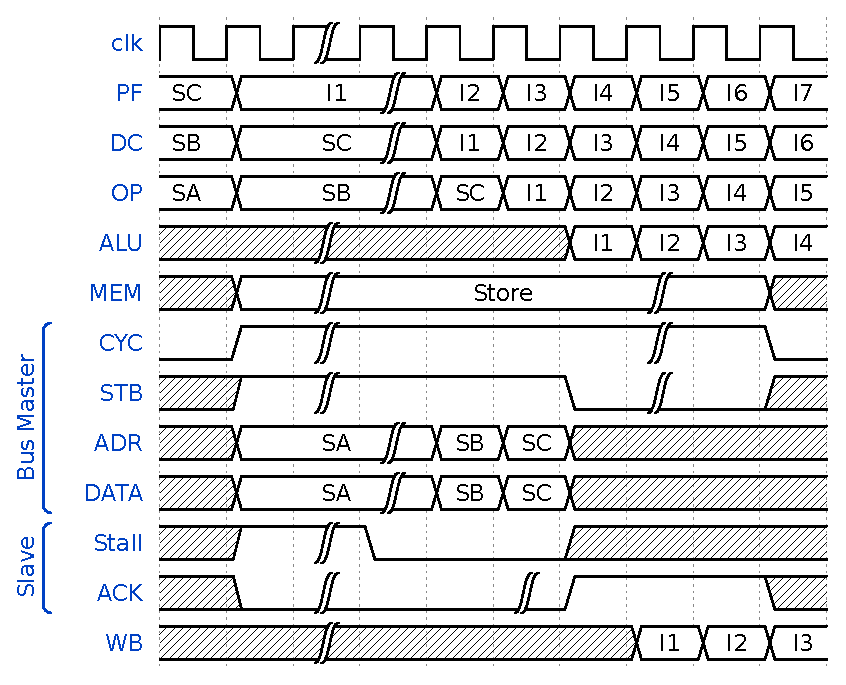
\includegraphics[width=4in]{../gfx/memwr.eps}
\caption{Pipeline handling of a store instruction}\label{fig:memwr}
\end{center}\end{figure}
since they can be busy with the bus without impacting later write back
pipeline stages.  Hence, only loads stall the pipeline.

This, of course, also assumes that the memory being accessed is a single cycle
memory and that there are no stalls to get to the memory.
Slower memories, such as the Quad SPI flash, will take longer--perhaps even
as long as forty clocks.   During this time the CPU and the external bus 
will be busy, and unable to do anything else.  Likewise, if it takes a couple
of clock cycles for the bus to be free, as shown in both Figs.~\ref{fig:memrd}
and~\ref{fig:memwr}, there will be stalls.

\item Memory operation followed by a memory operation
\begin{enumerate}
\item\ {\tt STO address,RA}
\item\ {\em (multiple stalls, bus dependent, 4 clocks best)}
\item\ {\tt LOD address,RB}
\item\ {\em (multiple stalls, bus dependent, 4 clocks best)}
\end{enumerate}

In this case, the LOD instruction cannot start until the STO is finished,
as illustrated by Fig.~\ref{fig:mstld}.
\begin{figure}\begin{center}
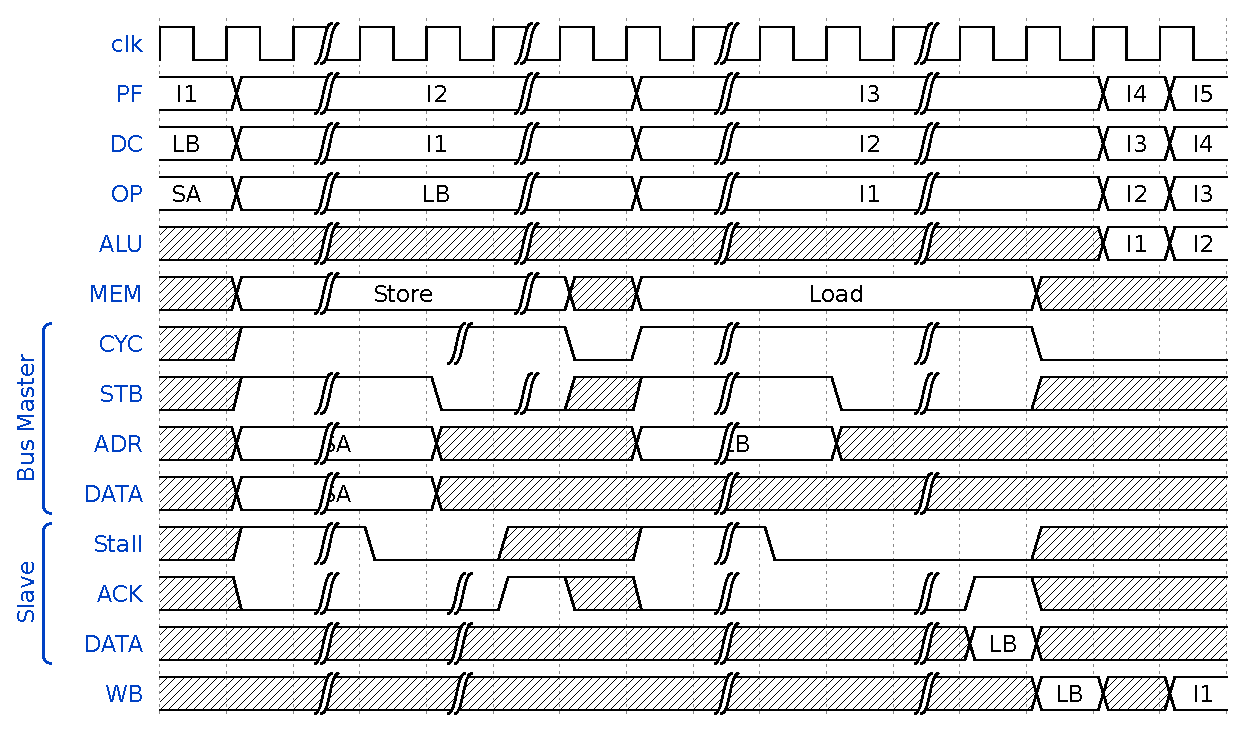
\includegraphics[width=5.5in]{../gfx/mstld.eps}
\caption{Pipeline handling of a store followed by a load instruction}\label{fig:mstld}
\end{center}\end{figure}
With proper scheduling, it is possible to do something in the ALU while the
memory unit is busy with the STO instruction, but otherwise this pipeline will
stall while waiting for it to complete before the load instruction can
start.

The Zip CPU does have the capability of supporting pipelined memory access,
but only under the following conditions: all accesses within the pipeline
must all be reads or all be writes, all must use the same register for their
address, and there can be no stalls or other instructions between pipelined
memory access instructions.  Further, the offset to memory must be increasing
by one address each instruction.  These conditions work well for saving or
storing registers to the stack.  Indeed, if you noticed, both
Fig.~\ref{fig:memrd} and Fig.~\ref{fig:memwr} illustrated pipelined memory
accesses.

\end{itemize}


\chapter{Peripherals}\label{chap:periph}

While the previous chapter describes a CPU in isolation, the Zip System
includes a minimum set of peripherals as well.  These peripherals are shown
in Fig.~\ref{fig:zipsystem}
\begin{figure}\begin{center}
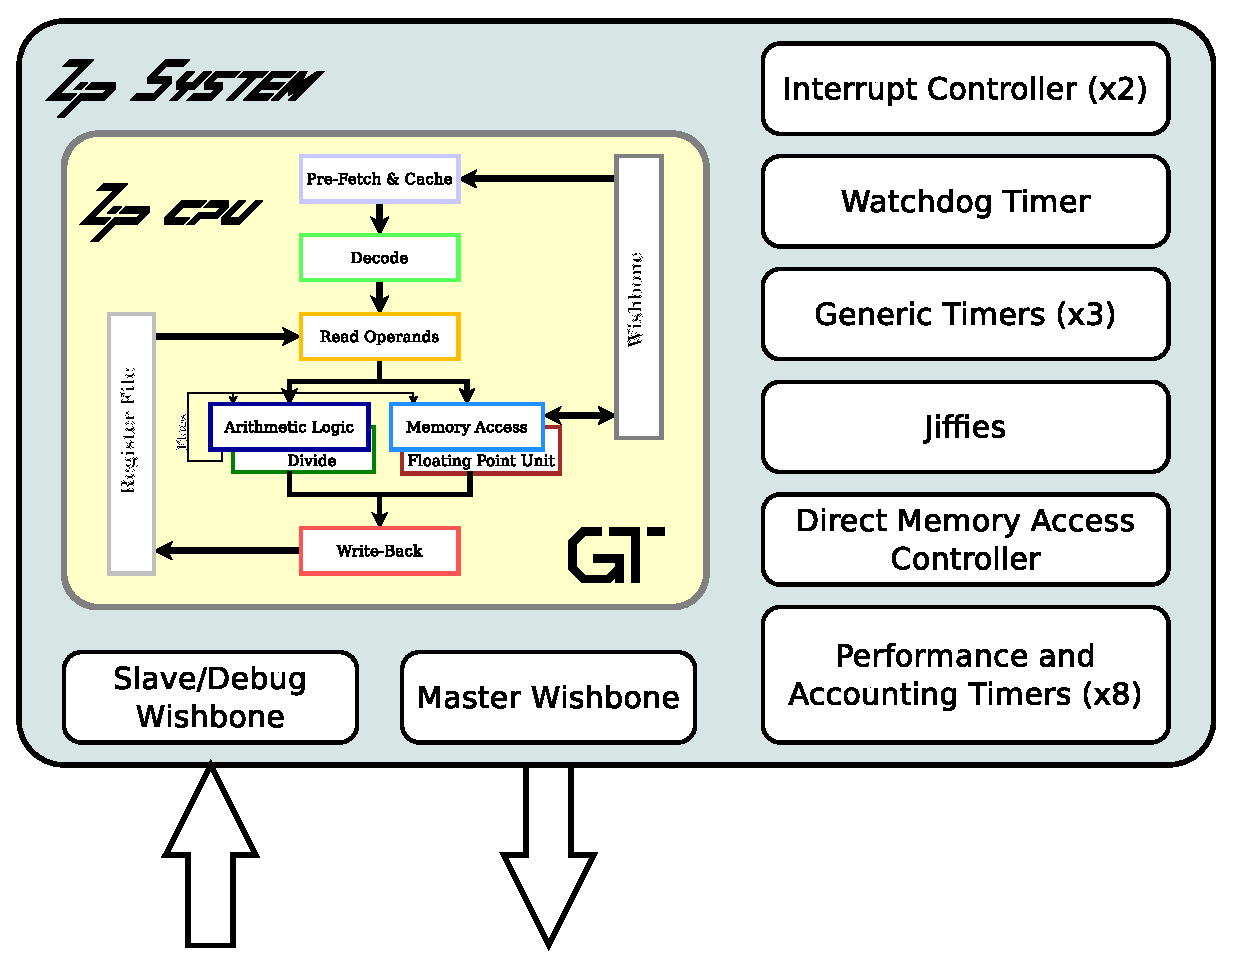
\includegraphics[width=3.5in]{../gfx/system.eps}
\caption{Zip System Peripherals}\label{fig:zipsystem}
\end{center}\end{figure}
and described here.  They are designed to make
the Zip CPU more useful in an Embedded Operating System environment.

\section{Interrupt Controller}\label{sec:pic}

Perhaps the most important peripheral within the Zip System is the interrupt
controller.  While the Zip CPU itself can only handle one interrupt, and has
only the one interrupt state: disabled or enabled, the interrupt controller
can make things more interesting.

The Zip System interrupt controller module supports up to 15 interrupts, all
controlled from one register.  Bit~31 of the interrupt controller controls
overall whether interrupts are enabled (1'b1) or disabled (1'b0).  Bits~16--30
control whether individual interrupts are enabled (1'b1) or disabled (1'b0).
Bit~15 is an indicator showing whether or not any interrupt is active, and 
bits~0--15 indicate whether or not an individual interrupt is active.

The interrupt controller has been designed so that bits can be controlled
individually without having any knowledge of the rest of the controller
setting.  To enable an interrupt, write to the register with the high order
global enable bit set and the respective interrupt enable bit set.  No other
bits will be affected.  To disable an interrupt, write to the register with
the high order global enable bit cleared and the respective interrupt enable
bit set.  To clear an interrupt, write a `1' to that interrupts status pin.
Zero's written to the register have no affect, save that a zero written to the
master enable will disable all interrupts.

As an example, suppose you wished to enable interrupt \#4.  You would then
write to the register a {\tt 0x80100010} to enable interrupt \#4 and to clear
any past active state.  When you later wish to disable this interrupt, you would
write a {\tt 0x00100010} to the register.  As before, this both disables the
interrupt and clears the active indicator.  This also has the side effect of
disabling all interrupts, so a second write of {\tt 0x80000000} may be necessary
to re-enable any other interrupts.

The Zip System currently hosts two interrupt controllers, a primary and a 
secondary.  The primary interrupt controller has one (or more) interrupt line(s)
which may come from an external interrupt source, and one interrupt line from
the secondary controller.  Other primary interrupts include the system timers,
the jiffies interrupt, and the manual cache interrupt.  The secondary interrupt
controller maintains an interrupt state for all of the processor accounting
counters.

\section{Counter}

The Zip Counter is a very simple counter: it just counts.  It cannot be
halted.  When it rolls over, it issues an interrupt.  Writing a value to the
counter just sets the current value, and it starts counting again from that
value.

Eight counters are implemented in the Zip System for process accounting.
This may change in the future, as nothing as yet uses these counters.

\section{Timer}

The Zip Timer is also very simple: it simply counts down to zero.  When it
transitions from a one to a zero it creates an interrupt.

Writing any non-zero value to the timer starts the timer.  If the high order
bit is set when writing to the timer, the timer becomes an interval timer and
reloads its last start time on any interrupt.  Hence, to mark seconds, one
might set the timer to 100~million (the number of clocks per second), and
set the high bit.  Ever after, the timer will interrupt the CPU once per
second (assuming a 100~MHz clock).  This reload capability also limits the
maximum timer value to $2^{31}-1$ (about 21~seconds using a 100~MHz clock),
rather than $2^{32}-1$.

\section{Watchdog Timer}

The watchdog timer is no different from any of the other timers, save for one
critical difference: the interrupt line from the watchdog
timer is tied to the reset line of the CPU.  Hence writing a `1' to the 
watchdog timer will always reset the CPU.  
To stop the Watchdog timer, write a `0' to it.  To start it,
write any other number to it---as with the other timers.

While the watchdog timer supports interval mode, it doesn't make as much sense
as it did with the other timers.

\section{Bus Watchdog}
There is an additional watchdog timer on the Wishbone bus.  This timer,
however, is hardware configured and not software configured.  The timer is
reset at the beginning of any bus transaction, and only counts clocks during
such bus transactions.  If the bus transaction takes longer than the number
of counts the timer allots, it will raise a bus error flag to terminate the
transaction.  This is useful in the case of any peripherals that are
misbehaving.  If the bus watchdog terminates a bus transaction, the CPU may
then read from its port to find out which memory location created the problem.

Aside from its unusual configuration, the bus watchdog is just another
implementation of the fundamental timer described above--stripped down
for simplicity.

\section{Jiffies}

This peripheral is motivated by the Linux use of `jiffies' whereby a process
can request to be put to sleep until a certain number of `jiffies' have
elapsed.  Using this interface, the CPU can read the number of `jiffies'
from the peripheral (it only has the one location in address space), add the
sleep length to it, and write the result back to the peripheral.  The
{\tt zipjiffies}
peripheral will record the value written to it only if it is nearer the current
counter value than the last current waiting interrupt time.  If no other 
interrupts are waiting, and this time is in the future, it will be enabled.
(There is currently no way to disable a jiffie interrupt once set, other
than to disable the interrupt line in the interrupt controller.)  The processor
may then place this sleep request into a list among other sleep requests.
Once the timer expires, it would write the next Jiffy request to the peripheral
and wake up the process whose timer had expired.

Indeed, the Jiffies register is nothing more than a glorified counter with
an interrupt.  Unlike the other counters, the Jiffies register cannot be set.
Writes to the jiffies register create an interrupt time.  When the Jiffies
register later equals the value written to it, an interrupt will be asserted
and the register then continues counting as though no interrupt had taken
place.

The purpose of this register is to support alarm times within a CPU.  To
set an alarm for a particular process $N$ clocks in advance, read the current
Jiffies value, and $N$, and write it back to the Jiffies register.  The
O/S must also keep track of values written to the Jiffies register.  Thus,
when an `alarm' trips, it should be removed from the list of alarms, the list
should be resorted, and the next alarm in terms of Jiffies should be written
to the register--possibly for a second time.

\section{Direct Memory Access Controller}

The Direct Memory Access (DMA) controller can be used to either move memory
from one location to another, to read from a peripheral into memory, or to
write from a peripheral into memory all without CPU intervention.  Further,
since the DMA controller can issue (and does issue) pipeline wishbone accesses,
any DMA memory move will by nature be faster than a corresponding program
accomplishing the same move.  To put this to numbers, it may take a program
18~clocks per word transferred, whereas this DMA controller can move one
word in eight clocks--provided it has bus access\footnote{The pipeline cost of 
the DMA controller, including setup cost, is a minimum of $14+2N$ clocks.}
(The CPU gets priority over the bus, but once bus access is granted to the
DMA peripheral, it will not be revoked mid--read or mid--write.)

When copying memory from one location to another, the DMA controller will
copy in units of a given transfer length--up to 1024 words at a time.  It will
read that transfer length into its internal buffer, and then write to the
destination address from that buffer.

When coupled with a peripheral, the DMA controller can be configured to start
a memory copy when any interrupt line goes high.  Further, the controller can
be configured to issue reads from (or to) the same address instead of
incrementing the address at each clock.  The DMA completes once the total
number of items specified (not the transfer length) have been transferred.

In each case, once the transfer is complete and the DMA unit returns to
idle, the DMA will issue an interrupt.


\chapter{Operation}\label{chap:ops}

The Zip CPU, and even the Zip System, is not a System on a Chip (SoC).  It 
needs to be connected to its operational environment in order to be used.
Specifically, some per system adjustments need to be made:
\begin{enumerate}
\item The Zip System depends upon an external 32-bit Wishbone bus.  This
	must exist, and must be connected to the Zip CPU for it to work.
\item The Zip System needs to be told of its {\tt RESET\_ADDRESS}.  This is
	the program counter of the first instruction following a reset.
\item To conserve logic, you'll want to set the {\tt ADDRESS\_WIDTH} parameter
	to the number of address bits on your wishbone bus.
\item Likewise, the {\tt LGICACHE} parameter sets the number of bits in
	the instruction cache address.  This means that the instruction cache
	will have $2^{\mbox{\tiny\tt LGICACHE}}$ locations within it.
\item If you want the Zip System to start up on its own, you will need to
	set the {\tt START\_HALTED} parameter to zero.  Otherwise, if you
	wish to manually start the CPU, that is if upon reset you want the
	CPU start start in its halted, reset state, then set this parameter to
	one.  This latter configuration is useful for a CPU that should be
	idle (i.e. halted) until given an explicit instruction from somewhere
	else to start.
\item The third parameter to set is the number of interrupts you will be
	providing from external to the CPU.  This can be anything from one
	to sixteen, but it cannot be zero.  (Set this to 1 and wire the single
	interrupt line to a 1'b0 if you do not wish to support any external
	interrupts.)
\item Finally, you need to place into some wishbone accessible address, whether
	RAM or (more likely) ROM, the initial instructions for the CPU.
\end{enumerate}
If you have enabled your CPU to start automatically, then upon power up the
CPU will immediately start executing your instructions, starting at the given
{\tt RESET\_ADDRESS}.

This is, however, not how I have used the Zip CPU.  I have instead used the
Zip CPU in a more controlled environment.  For me, the CPU starts in a 
halted state, and waits to be told to start.  Further, the RESET address is a
location in RAM.  After bringing up the board I am using, and further the
bus that is on it, the RAM memory is then loaded externally with the program
I wish the Zip System to run.  Once the RAM is loaded, I release the CPU.
The CPU then runs until either its halt condition or an exception occurrs in
supervisor mode, at which point its task is complete.

Eventually, I intend to place an operating system onto the ZipSystem, I'm 
just not there yet.

The rest of this chapter examines some common programming models, and how they
might be applied to the Zip System, and then finish with a couple of examples.

\section{System High}
The easiest and simplest way to run the Zip CPU is in the system high mode.
In this mode, the CPU runs your program in supervisor mode from reboot to
power down, and is never interrupted.  You will need to poll the interrupt
controller to determine when any external condition has become active.  This
mode is useful, and can handle many microcontroller tasks. 

Even better, in system high mode, all of the user registers are available
to the system high program as variables.  Accessing these registers can be
done in a single clock cycle, which would move them to the active register
set or move them back.  While this may seem like a load or store instruction,
none of these register accesses will suffer from memory delays.

The one thing that cannot be done in supervisor mode is a wait for interrupt
instruction.  This, however, is easily rectified by jumping to a user task
within the supervisors memory space, such as Tbl.~\ref{tbl:shi-idle}.
\begin{table}\begin{center}
\begin{tabbing}
{\tt supervisor\_idle:} \\
\hbox to 0.25in{}\={\em ; While not strictly required, the following move helps to} \\
\>	{\em ; ensure that the prefetch doesn't try to fetch an instruction} \\
\>	{\em ; outside of the CPU's address space when it switches to user} \\
\>	{\em ; mode.} \\
\>	{\tt MOV supervisor\_idle\_continue,uPC} \\
\>	{\em ; Put the processor into user mode and to sleep in the same} \\
\>	{\em ; instruction. } \\
\>	{\tt OR \$SLEEP|\$GIE,CC} \\
{\tt supervisor\_idle\_continue:} \\
\>	{\em ; Now, if we haven't done this inline, we need to return} \\
\>	{\em ; to whatever function called us.} \\
\>	{\tt RETN} \\
\end{tabbing}
\caption{Executing an idle from supervisor mode}\label{tbl:shi-idle}
\end{center}\end{table}

\section{Traditional Interrupt Handling}
Although the Zip CPU does not have a traditional interrupt architecture,
it is possible to create the more traditional interrupt approach via software.
In this mode, the programmable interrupt controller is used together with the
supervisor state to create the illusion of more traditional interrupt handling.

To set this up, upon reboot the supervisor task:
\begin{enumerate}
\item Creates a (single) user context, a user stack, and sets the user
	program counter to the entry of the user task
\item Creates a task table of ISR entries
\item Enables the master interrupt enable via the interrupt controller, albeit
	without enabling any of the fifteen potential underlying interrupts.
\item Switches to user mode, as the first part of the while loop in 
	Tbl.~\ref{tbl:traditional-isr}.
\end{enumerate}
\begin{table}\begin{center}
\begin{tabbing}
{\tt while(true) \{} \\
\hbox to 0.25in{}\= {\tt rtu();}\\
	\> {\tt if (trap) \{} {\em // Here, we allow users to install ISRs, or} \\
	\>\hbox to 0.25in{}\= {\em // whatever else they may wish to do in supervisor mode.} \\
	\> {\tt \} else \{} \\
	\> \> {\tt volatile int *pic = PIC\_ADDRESS;} \\
\\
	\> \> {\em // Save the user context before running any ISRs.  This could easily be}\\
	\> \> {\em // implemented as an inline assembly routine or macro}\\
	\> \> {\tt SAVE\_PARTIAL\_CONTEXT; }\\
	\> \> {\em // At this point, we know an interrupt has taken place:  Ask the programmable}\\
	\> \> {\em // interrupt controller (PIC) which interrupts are enabled and which are active.}\\
	\> \>	{\tt int	picv = *pic;}\\
	\> \>	{\em // Turn off all active interrupts}\\
	\> \>	{\em // Globally disable interrupt generation in the process}\\
	\> \>	{\tt int	active = (picv >> 16) \& picv \& 0x07fff;}\\
	\> \>	{\tt *pic = (active<<16);}\\
	\> \>	{\em // We build a mask of interrupts to re-enable in picv.}\\
	\> \>	{\tt picv = 0;}\\
	\> \>	{\tt for(int i=0,msk=1; i<15; i++, msk<<=1) \{}\\
	\> \>\hbox to 0.25in{}\={\tt if ((active \& msk)\&\&(isr\_table[i])) \{}\\
	\> \>\>\hbox to 0.25in{}\= {\tt mov(isr\_table[i],uPC); }\\
	\> \>\>\>	{\em // Acknowledge this particular interrupt.  While we could acknowledge all}\\
	\> \>\>\>	{\em // interrupts at once, by acknowledging only those with ISR's we allow}\\
	\> \>\>\>	{\em // the user process to use peripherals manually, and to manually check}\\
	\> \>\>\>	{\em // whether or no those other interrupts had occurred.}\\
	\> \>\>\>	{\tt *pic = msk; }\\
	\> \>\>\>	{\tt rtu(); }\\
	\> \>\>\>	{\em // The ISR will only exit on a trap in the Zip archtecture.  There is}\\
	\> \>\>\>	{\em // no {\tt RETI} instruction.  Since the PIC holds all interrupts disabled,}\\
	\> \>\>\>	{\em // there is no need to check for further interrupts.}\\
	\> \>\>\>	{\em // }\\
	\> \>\>\>	{\em // The tricky part is that, because of how the PIC is built, the ISR cannot}\\
	\>\>\>\>	{\em // re-enable its own interrupt without re-enabling all interrupts.  Hence, we}\\
	\>\>\>\>	{\em // look at R0 upon ISR completion to know if an interrupt needs to be }\\
	\> \>\>\>	{\em // re-enabled. }\\
	\> \>\>\>	{\tt mov(uR0,tmp); }\\
	\> \>\>\>	{\tt picv |= (tmp \& 0x7fff) << 16; }\\
	\> \>\>		{\tt \} }\\
	\> \>	{\tt \} }\\
	\> \>	{\tt RESTORE\_PARTIAL\_CONTEXT; }\\
	\> \>	{\em // Re-activate all (requested) interrupts }\\
	\> \>	{\tt *pic = picv | 0x80000000; }\\
	\>{\tt \} }\\
{\tt \}}\\
\end{tabbing}
\caption{Traditional Interrupt handling}\label{tbl:traditional-isr}
\end{center}\end{table}

We can work through the interrupt handling process by examining
Tbl.~\ref{tbl:traditional-isr}.  First, remember, the CPU is always running
either the user or the supervisor context.  Once the supervisor switches to
user mode, control does not return until either an interrupt or a trap
has taken place.  (Okay, there's also the possibility of a bus error, or an
illegal instruction such as an unimplemented floating point instruction---but
for now we'll just focus on the trap instruction.)  Therefore, if the trap bit
isn't set, then we know an interrupt has taken place.

To process an interrupt, we steal the user's stack: the PC and CC registers
are saved on the stack, as outlined in Tbl.~\ref{tbl:save-partial}.
\begin{table}\begin{center}
\begin{tabbing}
SAVE\_PARTIAL\_CONTEXT: \\
\hbox to 0.25in{}\= {\em ; We save R0, CC, and PC only} \\
\>        {\tt MOV -3(uSP),R3} \\
\>        {\tt MOV uR0,R0} \\
\>        {\tt MOV uCC,R1} \\
\>        {\tt MOV uPC,R2} \\
\>        {\tt STO R0,(R3)} {\em ; Exploit memory pipelining: }\\
\>        {\tt STO R1,1(R3)} {\em ; All instructions write to stack }\\
\>        {\tt STO R2,2(R3)} {\em ; All offsets increment by one }\\
\>        {\tt MOV R3,uSP} {\em ; Return the updated stack pointer } \\
\end{tabbing}
\caption{Example Saving Minimal User Context}\label{tbl:save-partial}
\end{center}\end{table}
This is much cheaper than the full context swap of a preemptive multitasking
kernel, but it also depends upon the ISR saving any state it uses.  Further,
if multiple ISR's get called at once, this looses its optimality property
very quickly.

As Sec.~\ref{sec:pic} discusses, the top of the PIC register stores which 
interrupts are enabled, and the bottom stores which have tripped.  (Interrupts
may trip without being enabled, they just will not generate an interrupt to the
CPU.)  Our first step is to query the register to find out our interrupt
state, and then to disable any interrupts that have tripped.  To do
that, we write a one to the enable half of the register while also clearing
the top bit (master interrupt enable).  This has the consequence of disabling
any and all further interrupts, not just the ones that have tripped.  Hence,
upon completion, we re--enable the master interrupt bit again.   Finally,
we keep track of which interrupts have tripped.

Using the bit mask of interrupts that have tripped, we walk through all fifteen
possible interrupts.  If there is an ISR installed, we acknowledge and reset
the interrupt within the PIC, and then call the ISR.  The ISR, however, cannot
re--enable its interrupt without re-enabling the master interrupt bit.  Thus,
to keep things simple, when the ISR is finished it places its interrupt
mask back into R0, or clears R0.  This tells the supervisor mode process which
interrupts to re--enable.  Any other registers that the ISR uses must be
saved and restored.  (This is only truly optimal if only a single ISR is
called.)  As a final instruction, the ISR clears the GIE bit executing a user
trap.  (Remember, the Zip CPU has no {\tt RETI} instruction to restore the
stack and return to userland.  It needs to go through the supervisor mode to
get there.)

Then, once all interrupts are handled, the user context is restored in  a 
fashion similar to Tbl.~\ref{tbl:restore-partial}.
\begin{table}\begin{center}
\begin{tabbing}
RESTORE\_PARTIAL\_CONTEXT: \\
\hbox to 0.25in{}\= {\em ; We retore R0, CC, and PC only} \\
\>        {\tt MOV uSP,R3} {\em ; Return the updated stack pointer } \\
\>        {\tt LOD R0,(R3),R0} {\em ; Exploit memory pipelining: }\\
\>        {\tt LOD R1,1(R3),R1} {\em ; All instructions write to stack }\\
\>        {\tt LOD R2,2(R3),R2} {\em ; All offsets increment by one }\\
\>        {\tt MOV R0,uR0} \\
\>        {\tt MOV R1,uCC} \\
\>        {\tt MOV R2,uPC} \\
\>        {\tt MOV 3(R3),uSP} \\
\end{tabbing}
\caption{Example Restoring Minimal User Context}\label{tbl:restore-partial}
\end{center}\end{table}
Again, this is short and sweet simply because any other registers that needed
saving were saved within the ISR.

There you have it: the Zip CPU, with its non-traditional interrupt architecture,
can still process interrupts in a very traditional fashion.

\section{Example: Idle Task}
One task every operating system needs is the idle task, the task that takes
place when nothing else can run.  On the Zip CPU, this task is quite simple,
and it is shown in assemble in Tbl.~\ref{tbl:idle-asm}.
\begin{table}\begin{center}
\begin{tabular}{ll}
{\tt idle\_task:} \\
&        {\em ; Wait for the next interrupt, then switch to supervisor task} \\
&        {\tt WAIT} \\
&        {\em ; When we come back, it's because the supervisor wishes to} \\
&        {\em ; wait for an interrupt again, so go back to the top.} \\
&        {\tt BRA idle\_task} \\
\end{tabular}
\caption{Example Idle Loop}\label{tbl:idle-asm}
\end{center}\end{table}
When this task runs, the CPU will fill up all of the pipeline stages up the
ALU.  The {\tt WAIT} instruction, upon leaving the ALU, places the CPU into
a sleep state where nothing more moves.  Sure, there may be some more settling,
the pipe cache continue to read until full, other instructions may issue until
the pipeline fills, but then everything will stall.  Then, once an interrupt
takes place, control passes to the supervisor task to handle the interrupt. 
When control passes back to this task, it will be on the next instruction.
Since that next instruction sends us back to the top of the task, the idle
task thus does nothing but wait for an interrupt.

This should be the lowest priority task, the task that runs when nothing else
can.  It will help lower the FPGA power usage overall---at least its dynamic
power usage.

\section{Example: Memory Copy}
One common operation is that of a memory move or copy.  Consider the C code
shown in Tbl.~\ref{tbl:memcp-c}.
\begin{table}\begin{center}
\parbox{4in}{\begin{tabbing}
{\tt void} \= {\tt memcp(void *dest, void *src, int len) \{} \\
	\> {\tt for(int i=0; i<len; i++)} \\
	\> \hspace{0.2in} {\tt *dest++ = *src++;} \\
\}
\end{tabbing}}
\caption{Example Memory Copy code in C}\label{tbl:memcp-c}
\end{center}\end{table}
This same code can be translated in Zip Assembly as shown in
Tbl.~\ref{tbl:memcp-asm}.
\begin{table}\begin{center}
\begin{tabular}{ll}
memcp: \\
&        {\em ; R0 = *dest, R1 = *src, R2 = LEN, R3 = return addr} \\
&        {\em ; The following will operate in $12N+19$ clocks.} \\
&        {\tt CMP 0,R2} \\ % 8 clocks per setup
&        {\tt MOV.Z R3,PC} {\em ; A conditional return }\\
&        {\tt SUB 1,SP} {\em ; Create a stack frame}\\
&        {\tt STO R4,(SP)} {\em ; and a local variable}\\
&        {\em ; (4 stalls, cannot be further scheduled away)} \\
loop: \\ % 12 clocks per loop
&        {\tt LOD (R1),R4} \\
&        {\em ; (4 stalls, cannot be scheduled away)} \\
&        {\tt STO R4,(R0)} {\em ; (4 schedulable stalls, has no impact now)} \\
&        {\tt SUB 1,R2} \\
&        {\tt BZ memcpend} \\
&        {\tt ADD 1,R0} \\
&        {\tt ADD 1,R1} \\
&        {\tt BRA loop} \\
&        {\em ; (1 stall on a BRA instruction)} \\
memcpend: % 11 clocks
&        {\tt LOD (SP),R4} \\
&        {\em ; (4 stalls, cannot be further scheduled away)} \\
&        {\tt ADD 1,SP} \\
&        {\tt JMP R3} \\
&        {\em ; (4 stalls)} \\
\end{tabular}
\caption{Example Memory Copy code in Zip Assembly}\label{tbl:memcp-asm}
\end{center}\end{table}
This example points out several things associated with the Zip CPU.  First,
a straightforward implementation of a for loop is not the fastest loop
structure.  For this reason, we have placed the test to continue at the
end.  Second, all pointers are {\tt void} pointers to arbitrary 32--bit
data types.  The Zip CPU does not have explicit support for smaller or larger
data types, and so this memory copy cannot be applied at a byte level.
Third, we've optimized the conditional jump to a return instruction into a
conditional return instruction.

\section{Example: Context Switch}

Fundamental to any multiprocessing system is the ability to switch from one
task to the next.  In the ZipSystem, this is accomplished in one of a couple
ways.  The first step is that an interrupt happens.  Anytime an interrupt 
happens, the CPU needs to execute the following tasks in supervisor mode:
\begin{enumerate}
\item Check for a trap instruction, or other user exception such as a break,
	bus error, division by zero error, or floating point exception.  That
	is, if the user process needs attending then we may not wish to adjust
	the context, check interrupts, or call the scheduler. 
	Tbl.~\ref{tbl:trap-check}
\begin{table}\begin{center}
\begin{tabular}{ll}
{\tt return\_to\_user:} \\
&	{\em; The instruction before the context switch processing must} \\
&	{\em; be the RTU instruction that enacted user mode in the first} \\
&	{\em; place.  We show it here just for reference.} \\
&	{\tt RTU} \\
{\tt trap\_check:} \\
&	{\tt MOV uCC,R0} \\
&	{\tt TST \$TRAP \textbar \$BUSERR \textbar \$DIVE \textbar \$FPE,R0} \\
&	{\tt BNZ swap\_out} \\
&	{; \em Do something here to execute the trap} \\
&	{; \em Don't need to call the scheduler, so we can just return} \\
&	{\tt BRA return\_to\_user} \\
\end{tabular}
\caption{Checking for whether the user task needs our attention}\label{tbl:trap-check}
\end{center}\end{table}
	shows the rudiments of this code, while showing nothing of how the
	actual trap would be implemented.
	
You may also wish to note that the instruction before the first instruction
in our context swap {\em must be} a return to userspace instruction. 
Remember, the supervisor process is re--entered where it left off.  This is
different from many other processors that enter interrupt mode at some vector
or other.  In this case, we always enter supervisor mode right where we last
left.\footnote{The one exception to this rule is upon reset where supervisor
mode is entered at a pre--programmed wishbone memory address.}

\item Capture user counters.  If the operating system is keeping track of
	system usage via the accounting counters, those counters need to be
	copied and accumulated into some master counter at this point.

\item Preserve the old context.  This involves pushing all the user registers
	onto the user stack and then copying the resulting stack address
	into the tasks task structure, as shown in Tbl.~\ref{tbl:context-out}.
\begin{table}\begin{center}
\begin{tabular}{ll}
{\tt swap\_out:} \\
&        {\tt MOV -15(uSP),R5} \\
&        {\tt STO R5,stack(R12)} \\
&        {\tt MOV uR0,R0} \\
&        {\tt MOV uR1,R1} \\
&        {\tt MOV uR2,R2} \\
&        {\tt MOV uR3,R3} \\
&        {\tt MOV uR4,R4} \\
&        {\tt STO R0,(R5)} {\em ; Exploit memory pipelining: }\\
&        {\tt STO R1,1(R5)} {\em ; All instructions write to stack }\\
&        {\tt STO R2,2(R5)} {\em ; All offsets increment by one }\\
&        {\tt STO R3,3(R5)} {\em ; Longest pipeline is 5 cycles.}\\
&        {\tt STO R4,4(R5)} \\
	& \ldots {\em ; Need to repeat for all user registers} \\
\iffalse
&        {\tt MOV uR5,R0} \\
&        {\tt MOV uR6,R1} \\
&        {\tt MOV uR7,R2} \\
&        {\tt MOV uR8,R3} \\
&        {\tt MOV uR9,R4} \\
&        {\tt STO R0,5(R5) }\\
&        {\tt STO R1,6(R5) }\\
&        {\tt STO R2,7(R5) }\\
&        {\tt STO R3,8(R5) }\\
&        {\tt STO R4,9(R5)} \\
\fi
&        {\tt MOV uR10,R0} \\
&        {\tt MOV uR11,R1} \\
&        {\tt MOV uR12,R2} \\
&        {\tt MOV uCC,R3} \\
&        {\tt MOV uPC,R4} \\
&        {\tt STO R0,10(R5)}\\
&        {\tt STO R1,11(R5)}\\
&        {\tt STO R2,12(R5)}\\
&        {\tt STO R3,13(R5)}\\
&        {\tt STO R4,14(R5)} \\
&	{\em ; We can skip storing the stack, uSP, since it'll be stored}\\
&	{\em ; elsewhere (in the task structure) }\\
\end{tabular}
\caption{Example Storing User Task Context}\label{tbl:context-out}
\end{center}\end{table}
For the sake of discussion, we assume the supervisor maintains a
pointer to the current task's structure in supervisor register
{\tt R12}, and that {\tt stack} is an offset to the beginning of this
structure indicating where the stack pointer is to be kept within it.

	For those who are still interested, the full code for this context
	save can be found as an assembler macro within the assembler
	include file, {\tt sys.i}.

\item Reset the watchdog timer.  If you are using the watchdog timer, it should
	be reset on a context swap, to know that things are still working.
	Example code for this is shown in Tbl.~\ref{tbl:reset-watchdog}.
\begin{table}\begin{center}
\begin{tabular}{ll}
\multicolumn{2}{l}{{\tt `define WATCHDOG\_ADDRESS 32'hc000\_0002}}\\
\multicolumn{2}{l}{{\tt `define WATCHDOG\_TICKS 32'd1\_000\_000} {; \em = 10 ms}}\\
&	{\tt LDI WATCHDOG\_ADDRESS,R0} \\
&	{\tt LDI WATCHDOG\_TICKS,R1} \\
&	{\tt STO R1,(R0)}
\end{tabular}
\caption{Example Watchdog Reset}\label{tbl:reset-watchdog}
\end{center}\end{table}

\item Interrupt handling.  An interrupt handler within the Zip System is nothing
	more than a task.  At context swap time, the supervisor needs to
	disable all of the interrupts that have tripped, and then enable
	all of the tasks that would deal with each of these interrupts.
	These can be user tasks, run at higher priority than any other user
	tasks.  Either way, they will need to re--enable their own interrupt
	themselves, if the interrupt is still relevant.

	An example of this master interrut handling is shown in 
	Tbl.~\ref{tbl:pre-handler}.
\begin{table}\begin{center}
\begin{tabular}{ll}
{\tt pre\_handler:} \\
&	{\tt LDI PIC\_ADDRESS,R0 } \\
&	{\em ; Start by grabbing the interrupt state from the interrupt}\\
&	{\em ; controller.  We'll store this into the register R7 so that }\\
&	{\em ; we can keep and preserve this information for the scheduler}\\
&	{\em ; to use later. }\\
&	{\tt LOD (R0),R1} \\
&	{\tt MOV R1,R7 } \\
&	{\em ; As a next step, we need to acknowledge and disable all active}\\
&	{\em ; interrupts. We'll start by calculating all of our active}\\
&	{\em ; interrupts.}\\
&	{\tt AND 0x07fff,R1 } \\
&	{\em ; Put the active interrupts into the upper half of R1} \\
&	{\tt ROL 16,R1 } \\
&	{\tt LDILO 0x0ffff,R1	} \\
&	{\tt AND R7,R1}\\
&	{\em ; Acknowledge and disable active interrupts}\\
&	{\em ; This also disables all interrupts from the controller, so}\\
&	{\em ; we'll need to re-enable interrupts in general shortly } \\
&	{\tt STO R1,(R0) } \\
&	{\em ; We leave our active interrupt mask in R7 so the scheduler can}\\
&	{\em ; release any tasks that depended upon them. } \\
\end{tabular}
\caption{Example checking for active interrupts}\label{tbl:pre-handler}
\end{center}\end{table}

\item Calling the scheduler.  This needs to be done to pick the next task
	to switch to.  It may be an interrupt handler, or it may  be a normal
	user task.  From a priority standpoint, it would make sense that the
	interrupt handlers all have a higher priority than the user tasks,
	and that once they have been called the user tasks may then be called
	again.  If no task is ready to run, run the idle task to wait for an
	interrupt.

	This suggests a minimum of four task priorities:
	\begin{enumerate}
	\item Interrupt handlers, executed with their interrupts disabled
	\item Device drivers, executed with interrupts re-enabled
	\item User tasks
	\item The idle task, executed when nothing else is able to execute
	\end{enumerate}

	For our purposes here, we'll just assume that a pointer to the current
	task is maintained in {\tt R12}, that a {\tt JSR scheduler} is 
	called, and that the next current task is likewise placed into
	{\tt R12}.

\item Restore the new tasks context.  Given that the scheduler has returned a
	task that can be run at this time, the stack pointer needs to be 
	pulled out of the tasks task structure, placed into the user
	register, and then the rest of the user registers need to be popped
	back off of the stack to run this task.  An example of this is
	shown in Tbl.~\ref{tbl:context-in},
\begin{table}\begin{center}
\begin{tabular}{ll}
{\tt swap\_in:} \\
&	{\tt LOD stack(R12),R5} \\
&	{\tt MOV 15(R1),uSP} \\
	& {\em ; Be sure to exploit the memory pipelining capability} \\
&	{\tt LOD (R5),R0} \\
&	{\tt LOD 1(R5),R1} \\
&	{\tt LOD 2(R5),R2} \\
&	{\tt LOD 3(R5),R3} \\
&	{\tt LOD 4(R5),R4} \\
&	{\tt MOV R0,uR0} \\
&	{\tt MOV R1,uR1} \\
&	{\tt MOV R2,uR2} \\
&	{\tt MOV R3,uR3} \\
&	{\tt MOV R4,uR4} \\
	& \ldots {\em ; Need to repeat for all user registers} \\
&	{\tt LOD 10(R5),R0} \\
&	{\tt LOD 11(R5),R1} \\
&	{\tt LOD 12(R5),R2} \\
&	{\tt LOD 13(R5),R3} \\
&	{\tt LOD 14(R5),R4} \\
&	{\tt MOV R0,uR10} \\
&	{\tt MOV R1,uR11} \\
&	{\tt MOV R2,uR12} \\
&	{\tt MOV R3,uCC} \\
&	{\tt MOV R4,uPC} \\

&	{\tt BRA return\_to\_user} \\
\end{tabular}
\caption{Example Restoring User Task Context}\label{tbl:context-in}
\end{center}\end{table}
	assuming as before that the task
	pointer is found in supervisor register {\tt R12}.
	As with storing the user context, the full code associated with
	restoring the user context can be found in the assembler include
	file, {\tt sys.i}.

\item Clear the userspace accounting registers.  In order to keep track of
	per process system usage, these registers need to be cleared before
	reactivating the userspace process.  That way, upon the next
	interrupt, we'll know how many clocks the userspace program has
	encountered, and how many instructions it was able to issue in
	those many clocks. 

\item Jump back to the instruction just before saving the last tasks context,
	because that location in memory contains the return from interrupt
	command that we are going to need to execute, in order to guarantee
	that we return back here again.
\end{enumerate}

\chapter{Application Binary Interface}\label{chap:abi}
% ELF Format
% Stack:
%	R13 is the stack register.
%	The stack grows downward.
%	Memory at the current stack pointer is allocated.
%	Hence, a PUSH is : SUB 1,SP; STO Rx,(SP)
% Heap:
%	In general, not yet implemented.  
%	A less than adequate Heap has been implemented as a pointer, from which
%	malloc requests simply decrement it.  Free's are NOOPs, leaving
%	allocated memory allocated forever.
% Call/JSR format:
%	First 4 operands in registers, rest on the stack
%	The return address is passed in R0
% Builtin functions:
%	zip_halt();
%	zip_system();
%	zip_wait();
%	zip_rtu();
%	zip_break();
%	zip_busy();
%	zip_idle();
%	zip_syscall(a,b,c,d)
%	zip_save_context(*)
%	zip_restore_context(*)
%	int zip_bitrev(int);
%	int zip_cc();
%	int zip_ucc();
%
% Address layout:
%	Yet undefined.
%
% The need for a linker file
%	No requirement has (yet) been made for address layout.  As a result,
%	every different ZipCPU implementation needs a (new) linker definition
%	file, since peripherals, memory, and so on may move between
%	implementations.
%
%	Since every implementation can have memory at different addresses,
%	the ZipCPU does not (yet) have a default linker file.
\chapter{Registers}\label{chap:regs}

The ZipSystem registers fall into two categories, ZipSystem internal registers
accessed via the ZipCPU shown in Tbl.~\ref{tbl:zpregs},
\begin{table}[htbp]
\begin{center}\begin{reglist}
PIC   & \scalebox{0.8}{\tt 0xc0000000} & 32 & R/W & Primary Interrupt Controller \\\hline
WDT   & \scalebox{0.8}{\tt 0xc0000001} & 32 & R/W & Watchdog Timer \\\hline
  & \scalebox{0.8}{\tt 0xc0000002} & 32 & R & Address of last bus error \\\hline
CTRIC & \scalebox{0.8}{\tt 0xc0000003} & 32 & R/W & Secondary Interrupt Controller \\\hline
TMRA  & \scalebox{0.8}{\tt 0xc0000004} & 32 & R/W & Timer A\\\hline
TMRB  & \scalebox{0.8}{\tt 0xc0000005} & 32 & R/W & Timer B\\\hline
TMRC  & \scalebox{0.8}{\tt 0xc0000006} & 32 & R/W & Timer C\\\hline
JIFF  & \scalebox{0.8}{\tt 0xc0000007} & 32 & R/W & Jiffies \\\hline
MTASK  & \scalebox{0.8}{\tt 0xc0000008} & 32 & R/W & Master Task Clock Counter \\\hline
MMSTL  & \scalebox{0.8}{\tt 0xc0000009} & 32 & R/W & Master Stall Counter \\\hline
MPSTL  & \scalebox{0.8}{\tt 0xc000000a} & 32 & R/W & Master Pre--Fetch Stall Counter \\\hline
MICNT  & \scalebox{0.8}{\tt 0xc000000b} & 32 & R/W & Master Instruction Counter\\\hline
UTASK  & \scalebox{0.8}{\tt 0xc000000c} & 32 & R/W & User Task Clock Counter \\\hline
UMSTL  & \scalebox{0.8}{\tt 0xc000000d} & 32 & R/W & User Stall Counter \\\hline
UPSTL  & \scalebox{0.8}{\tt 0xc000000e} & 32 & R/W & User Pre--Fetch Stall Counter \\\hline
UICNT  & \scalebox{0.8}{\tt 0xc000000f} & 32 & R/W & User Instruction Counter\\\hline
DMACTRL  & \scalebox{0.8}{\tt 0xc0000010} & 32 & R/W & DMA Control Register\\\hline
DMALEN  & \scalebox{0.8}{\tt 0xc0000011} & 32 & R/W & DMA total transfer length\\\hline
DMASRC  & \scalebox{0.8}{\tt 0xc0000012} & 32 & R/W & DMA source address\\\hline
DMADST  & \scalebox{0.8}{\tt 0xc0000013} & 32 & R/W & DMA destination address\\\hline
% Cache  & \scalebox{0.8}{\tt 0xc0100000} & & & Base address of the Cache memory\\\hline
\end{reglist}
\caption{Zip System Internal/Peripheral Registers}\label{tbl:zpregs}
\end{center}\end{table}
and the two debug registers shown in Tbl.~\ref{tbl:dbgregs}.
\begin{table}[htbp]
\begin{center}\begin{reglist}
ZIPCTRL & 0 & 32 & R/W & Debug Control Register \\\hline
ZIPDATA & 1 & 32 & R/W & Debug Data Register \\\hline
\end{reglist}
\caption{Zip System Debug Registers}\label{tbl:dbgregs}
\end{center}\end{table}

\section{Peripheral Registers}
The peripheral registers, listed in Tbl.~\ref{tbl:zpregs}, are shown in the
CPU's address space.  These may be accessed by the CPU at these addresses,
and when so accessed will respond as described in Chapt.~\ref{chap:periph}.
These registers will be discussed briefly again here.

\subsection{Interrupt Controller(s)}
The Zip CPU Interrupt controller has four different types of bits, as shown in 
Tbl.~\ref{tbl:picbits}.
\begin{table}\begin{center}
\begin{bitlist}
31 & R/W & Master Interrupt Enable\\\hline
30\ldots 16 & R/W & Interrupt Enables, write `1' to change\\\hline
15 & R & Current Master Interrupt State\\\hline
15\ldots 0 & R/W & Input Interrupt states, write `1' to clear\\\hline
\end{bitlist}
\caption{Interrupt Controller Register Bits}\label{tbl:picbits}
\end{center}\end{table}
The high order bit, or bit--31, is the master interrupt enable bit.  When this
bit is set, then any time an interrupt occurs the CPU will be interrupted and
will switch to supervisor mode, etc.  

Bits 30~\ldots 16 are interrupt enable bits.  Should the interrupt line go
hi while enabled, an interrupt will be generated.  (All interrupts are positive
edge triggered.)  To set an interrupt enable bit, one needs to write the
master interrupt enable while writing a `1' to this the bit.  To clear, one
need only write a `0' to the master interrupt enable, while leaving this line
high.  

Bits 15\ldots 0 are the current state of the interrupt vector.  Interrupt lines
trip when they go high, and remain tripped until they are acknowledged.  If
the interrupt goes high for longer than one pulse, it may be high when a clear
is requested.  If so, the interrupt will not clear.  The line must go low
again before the status bit can be cleared.

As an example, consider the following scenario where the Zip CPU supports four
interrupts, 3\ldots0.
\begin{enumerate}
\item The Supervisor will first, while in the interrupts disabled mode,
	write a {\tt 32'h800f000f} to the controller.  The supervisor may then
	switch to the user state with interrupts enabled.
\item When an interrupt occurs, the supervisor will switch to the interrupt
	state.  It will then cycle through the interrupt bits to learn which
	interrupt handler to call.
\item If the interrupt handler expects more interrupts, it will clear its
	current interrupt when it is done handling the interrupt in question.
	To do this, it will write a `1' to the low order interrupt mask,
	such as writing a {\tt 32'h0000\_0001}.
\item If the interrupt handler does not expect any more interrupts, it will
	instead clear the interrupt from the controller by writing a 
	{\tt 32'h0001\_0001} to the controller.
\item Once all interrupts have been handled, the supervisor will write a
	{\tt 32'h8000\_0000} to the interrupt register to re-enable interrupt
	generation.
\item The supervisor should also check the user trap bit, and possible soft
	interrupt bits here, but this action has nothing to do with the
	interrupt control register.
\item The supervisor will then leave interrupt mode, possibly adjusting
	whichever task is running, by executing a return from interrupt
	command.
\end{enumerate}

\subsection{Timer Register}

Leaving the interrupt controller, we show the timer registers bit definitions
in Tbl.~\ref{tbl:tmrbits}.
\begin{table}\begin{center}
\begin{bitlist}
31 & R/W & Auto-Reload\\\hline
30\ldots 0 & R/W & Current timer value\\\hline
\end{bitlist}
\caption{Timer Register Bits}\label{tbl:tmrbits}
\end{center}\end{table}
As you may recall, the timer just counts down to zero and then trips an
interrupt.  Writing to the current timer value sets that value, and reading
from it returns that value.  Writing to the current timer value while also
setting the auto--reload bit will send the timer into an auto--reload mode.
In this mode, upon setting its interrupt bit for one cycle, the timer will
also reset itself back to the value of the timer that was written to it when
the auto--reload option was written to it.  To clear and stop the timer, 
just simply write a `32'h00' to this register.

\subsection{Jiffies}

The Jiffies register is somewhat similar in that the register always changes.
In this case, the register counts up, whereas the timer always counted down.
Reads from this register, as shown in Tbl.~\ref{tbl:jiffybits},
\begin{table}\begin{center}
\begin{bitlist}
31\ldots 0 & R & Current jiffy value\\\hline
31\ldots 0 & W & Value/time of next interrupt\\\hline
\end{bitlist}
\caption{Jiffies Register Bits}\label{tbl:jiffybits}
\end{center}\end{table}
always return the time value contained in the register.  Writes greater than
the current Jiffy value, that is where the new value minus the old value is
greater than zero while ignoring truncation, will set a new Jiffy interrupt
time.  At that time, the Jiffy vector will clear, and another interrupt time
may either be written to it, or it will just continue counting without
activating any more interrupts.

\subsection{Performance Counters}

The Zip CPU also supports several counter peripherals, mostly in the way of
process accounting.  This peripherals have a single register associated with
them, shown in Tbl.~\ref{tbl:ctrbits}.
\begin{table}\begin{center}
\begin{bitlist}
31\ldots 0 & R/W & Current counter value\\\hline
\end{bitlist}
\caption{Counter Register Bits}\label{tbl:ctrbits}
\end{center}\end{table}
Writes to this register set the new counter value.  Reads read the current
counter value.  

The current design operation of these counters is that of performance counting.
Two sets of four registers are available for keeping track of performance.
The first is a task counter.  This just counts clock ticks.  The second
counter is a prefetch stall counter, then an master stall counter.  These
allow the CPU to be evaluated as to how efficient it is.  The fourth and
final counter is an instruction counter, which counts how many instructions the
CPU has issued.

It is envisioned that these counters will be used as follows: First, every time
a master counter rolls over, the supervisor (Operating System) will record
the fact.  Second, whenever activating a user task, the Operating System will
set the four user counters to zero.  When the user task has completed, the
Operating System will read the timers back off, to determine how much of the
CPU the process had consumed.  To keep this accurate, the user counters will
only increment when the GIE bit is set to indicate that the processor is
in user mode.

\subsection{DMA Controller}

The final peripheral to discuss is the DMA controller.  This controller
has four registers.  Of these four, the length, source and destination address
registers should need no further explanation.  They are full 32--bit registers
specifying the entire transfer length, the starting address to read from, and
the starting address to write to.  The registers can be written to when the
DMA is idle, and read at any time.  The control register, however, will need
some more explanation.

The bit allocation of the control register is shown in Tbl.~\ref{tbl:dmacbits}.
\begin{table}\begin{center}
\begin{bitlist}
31 & R & DMA Active\\\hline
30 & R & Wishbone error, transaction aborted.  This bit is cleared the next time
	this register is written to.\\\hline
29 & R/W & Set to `1' to prevent the controller from incrementing the source address, `0' for normal memory copy. \\\hline
28 & R/W & Set to `1' to prevent the controller from incrementing the
	destination address, `0' for normal memory copy. \\\hline
27 \ldots 16 & W & The DMA Key.  Write a 12'hfed to these bits to start the
	activate any DMA transfer.  \\\hline
27 & R & Always reads `0', to force the deliberate writing of the key. \\\hline
26 \ldots 16 & R & Indicates the number of items in the transfer buffer that
	have yet to be written. \\\hline
15 & R/W & Set to `1' to trigger on an interrupt, or `0' to start immediately
	upon receiving a valid key.\\\hline
14\ldots 10 & R/W & Select among one of 32~possible interrupt lines.\\\hline
9\ldots 0 & R/W & Intermediate transfer length minus one.  Thus, to transfer
	one item at a time set this value to 0. To transfer 1024 at a time,
	set it to 1023.\\\hline
\end{bitlist}
\caption{DMA Control Register Bits}\label{tbl:dmacbits}
\end{center}\end{table}
This control register has been designed so that the common case of memory
access need only set the key and the transfer length.  Hence, writing a
\hbox{32'h0fed03ff} to the control register will start any memory transfer.  
On the other hand, if you wished to read from a serial port (constant address)
and put the result into a buffer every time a word was available, you 
might wish to write \hbox{32'h2fed8000}--this assumes, of course, that you
have a serial port wired to the zero bit of this interrupt control.  (The
DMA controller does not use the interrupt controller, and cannot clear
interrupts.)  As a third example, if you wished to write to an external
FIFO anytime it was less than half full (had fewer than 512 items), and
interrupt line 3 indicated this condition, you might wish to issue a
\hbox{32'h1fed8dff} to this port.

\section{Debug Port Registers}
Accessing the Zip System via the debug port isn't as straight forward as
accessing the system via the wishbone bus.  The debug port itself has been
reduced to two addresses, as outlined earlier in Tbl.~\ref{tbl:dbgregs}.
Access to the Zip System begins with the Debug Control register, shown in 
Tbl.~\ref{tbl:dbgctrl}.
\begin{table}\begin{center}
\begin{bitlist}
31\ldots 14 & R & External interrupt state.  Bit 14 is valid for one
	interrupt only, bit 15 for two, etc.\\\hline
13 & R & CPU GIE setting\\\hline
12 & R & CPU is sleeping\\\hline
11 & W & Command clear PF cache\\\hline
10 & R/W & Command HALT, Set to `1' to halt the CPU\\\hline
9 & R & Stall Status, `1' if CPU is busy (i.e., not halted yet)\\\hline
8 & R/W & Step Command, set to `1' to step the CPU, also sets the halt bit\\\hline
7 & R & Interrupt Request Pending\\\hline
6 & R/W & Command RESET \\\hline
5\ldots 0 & R/W & Debug Register Address \\\hline
\end{bitlist}
\caption{Debug Control Register Bits}\label{tbl:dbgctrl}
\end{center}\end{table}

The first step in debugging access is to determine whether or not the CPU
is halted, and to halt it if not.  To do this, first write a `1' to the
Command HALT bit.  This will halt the CPU and place it into debug mode.
Once the CPU is halted, the stall status bit will drop to zero.  Thus,
if bit 10 is high and bit 9 low, the debug port is open to examine the 
internal state of the CPU.

At this point, the external debugger may examine internal state information
from within the CPU.  To do this, first write again to the command register
a value (with command halt still high) containing the address of an internal
register of interest in the bottom 6~bits.  Internal registers that may be
accessed this way are listed in Tbl.~\ref{tbl:dbgaddrs}.
\begin{table}\begin{center}
\begin{reglist}
sR0 & 0 & 32 & R/W & Supervisor Register R0 \\\hline
sR1 & 0 & 32 & R/W & Supervisor Register R1 \\\hline
sSP & 13 & 32 & R/W & Supervisor Stack Pointer\\\hline
sCC & 14 & 32 & R/W & Supervisor Condition Code Register \\\hline
sPC & 15 & 32 & R/W & Supervisor Program Counter\\\hline
uR0 & 16 & 32 & R/W & User Register R0 \\\hline
uR1 & 17 & 32 & R/W & User Register R1 \\\hline
uSP & 29 & 32 & R/W & User Stack Pointer\\\hline
uCC & 30 & 32 & R/W & User Condition Code Register \\\hline
uPC & 31 & 32 & R/W & User Program Counter\\\hline
PIC & 32 & 32 & R/W & Primary Interrupt Controller \\\hline
WDT & 33 & 32 & R/W & Watchdog Timer\\\hline
BUS & 34 & 32 & R & Last Bus Error\\\hline
CTRIC & 35 & 32 & R/W & Secondary Interrupt Controller\\\hline
TMRA & 36 & 32 & R/W & Timer A\\\hline
TMRB & 37 & 32 & R/W & Timer B\\\hline
TMRC & 38 & 32 & R/W & Timer C\\\hline
JIFF & 39 & 32 & R/W & Jiffies peripheral\\\hline
MTASK & 40 & 32 & R/W & Master task clock counter\\\hline
MMSTL & 41 & 32 & R/W & Master memory stall counter\\\hline
MPSTL & 42 & 32 & R/W & Master Pre-Fetch Stall counter\\\hline
MICNT & 43 & 32 & R/W & Master instruction counter\\\hline
UTASK & 44 & 32 & R/W & User task clock counter\\\hline
UMSTL & 45 & 32 & R/W & User memory stall counter\\\hline
UPSTL & 46 & 32 & R/W & User Pre-Fetch Stall counter\\\hline
UICNT & 47 & 32 & R/W & User instruction counter\\\hline
DMACMD & 48 & 32 & R/W & DMA command and status register\\\hline
DMALEN & 49 & 32 & R/W & DMA transfer length\\\hline
DMARD & 50 & 32 & R/W & DMA read address\\\hline
DMAWR & 51 & 32 & R/W & DMA write address\\\hline
\end{reglist}
\caption{Debug Register Addresses}\label{tbl:dbgaddrs}
\end{center}\end{table}
Primarily, these ``registers'' include access to the entire CPU register
set, as well as the internal peripherals.  To read one of these registers
once the address is set, simply issue a read from the data port.  To write
one of these registers or peripheral ports, simply write to the data port
after setting the proper address.

In this manner, all of the CPU's internal state may be read and adjusted.

As an example of how to use this, consider what would happen in the case
of an external break point.  If and when the CPU hits a break point that
causes it to halt, the Command HALT bit will activate on its own, the CPU
will then raise an external interrupt line and wait for a debugger to examine
its state.  After examining the state, the debugger will need to remove
the breakpoint by writing a different instruction into memory and by writing
to the command register while holding the clear cache, command halt, and
step CPU bits high, (32'hd00).  The debugger may then replace the breakpoint
now that the CPU has gone beyond it, and clear the cache again (32'h500).

To leave this debug mode, simply write a `32'h0' value to the command register.

\chapter{Wishbone Datasheets}\label{chap:wishbone}
The Zip System supports two wishbone ports, a slave debug port and a master
port for the system itself.  These are shown in Tbl.~\ref{tbl:wishbone-slave}
\begin{table}[htbp]
\begin{center}
\begin{wishboneds}
Revision level of wishbone & WB B4 spec \\\hline
Type of interface & Slave, Read/Write, single words only \\\hline
Address Width & 1--bit \\\hline
Port size & 32--bit \\\hline
Port granularity & 32--bit \\\hline
Maximum Operand Size & 32--bit \\\hline
Data transfer ordering & (Irrelevant) \\\hline
Clock constraints & Works at 100~MHz on a Basys--3 board, and 80~MHz on a
		XuLA2--LX25\\\hline
Signal Names & \begin{tabular}{ll}
		Signal Name & Wishbone Equivalent \\\hline
		{\tt i\_clk} & {\tt CLK\_I} \\
		{\tt i\_dbg\_cyc} & {\tt CYC\_I} \\
		{\tt i\_dbg\_stb} & {\tt STB\_I} \\
		{\tt i\_dbg\_we} & {\tt WE\_I} \\
		{\tt i\_dbg\_addr} & {\tt ADR\_I} \\
		{\tt i\_dbg\_data} & {\tt DAT\_I} \\
		{\tt o\_dbg\_ack} & {\tt ACK\_O} \\
		{\tt o\_dbg\_stall} & {\tt STALL\_O} \\
		{\tt o\_dbg\_data} & {\tt DAT\_O}
		\end{tabular}\\\hline
\end{wishboneds}
\caption{Wishbone Datasheet for the Debug Interface}\label{tbl:wishbone-slave}
\end{center}\end{table}
and Tbl.~\ref{tbl:wishbone-master} respectively.
\begin{table}[htbp]
\begin{center}
\begin{wishboneds}
Revision level of wishbone & WB B4 spec \\\hline
Type of interface & Master, Read/Write, single cycle or pipelined\\\hline
Address Width & (Zip System parameter, can be up to 32--bit bits) \\\hline
Port size & 32--bit \\\hline
Port granularity & 32--bit \\\hline
Maximum Operand Size & 32--bit \\\hline
Data transfer ordering & (Irrelevant) \\\hline
Clock constraints & Works at 100~MHz on a Basys--3 board, and 80~MHz on a
		XuLA2--LX25\\\hline
Signal Names & \begin{tabular}{ll}
		Signal Name & Wishbone Equivalent \\\hline
		{\tt i\_clk} & {\tt CLK\_O} \\
		{\tt o\_wb\_cyc} & {\tt CYC\_O} \\
		{\tt o\_wb\_stb} & {\tt STB\_O} \\
		{\tt o\_wb\_we} & {\tt WE\_O} \\
		{\tt o\_wb\_addr} & {\tt ADR\_O} \\
		{\tt o\_wb\_data} & {\tt DAT\_O} \\
		{\tt i\_wb\_ack} & {\tt ACK\_I} \\
		{\tt i\_wb\_stall} & {\tt STALL\_I} \\
		{\tt i\_wb\_data} & {\tt DAT\_I} \\
		{\tt i\_wb\_err} & {\tt ERR\_I}
		\end{tabular}\\\hline
\end{wishboneds}
\caption{Wishbone Datasheet for the CPU as Master}\label{tbl:wishbone-master}
\end{center}\end{table}
I do not recommend that you connect these together through the interconnect.
Rather, the debug port of the CPU should be accessible regardless of the state
of the master bus.

You may wish to notice that neither the {\tt LOCK} nor the {\tt RTY} (retry)
wires have been connected to the CPU's master interface.  If necessary, a
rudimentary {\tt LOCK} may be created by tying the wire to the {\tt wb\_cyc}
line.  As for the {\tt RTY}, all the CPU recognizes at this point are bus
errors---it cannot tell the difference between a temporary and a permanent bus
error.

\chapter{Clocks}\label{chap:clocks}

This core is based upon the Basys--3 development board sold by Digilent. 
The Basys--3 development board contains one external 100~MHz clock, which is
sufficient to run the Zip CPU core.
\begin{table}[htbp]
\begin{center}
\begin{clocklist}
i\_clk & External & 100~MHz & 100~MHz & System clock.\\\hline
\end{clocklist}
\caption{List of Clocks}\label{tbl:clocks}
\end{center}\end{table}
I hesitate to suggest that the core can run faster than 100~MHz, since I have
had struggled with various timing violations to keep it at 100~MHz.  So, for 
now, I will only state that it can run at 100~MHz.

On a SPARTAN 6, the clock can run successfully at 80~MHz.

\chapter{I/O Ports}\label{chap:ioports}
The I/O ports to the Zip CPU may be grouped into three categories.  The first
is that of the master wishbone used by the CPU, then the slave wishbone used
to command the CPU via a debugger, and then the rest.  The first two of these
were already discussed in the wishbone chapter.  They are listed here
for completeness in Tbl.~\ref{tbl:iowb-master}
\begin{table}
\begin{center}\begin{portlist}
{\tt o\_wb\_cyc}   &  1 & Output & Indicates an active Wishbone cycle\\\hline
{\tt o\_wb\_stb}   &  1 & Output & WB Strobe signal\\\hline
{\tt o\_wb\_we}    &  1 & Output & Write enable\\\hline
{\tt o\_wb\_addr}  & 32 & Output & Bus address \\\hline
{\tt o\_wb\_data}  & 32 & Output & Data on WB write\\\hline
{\tt i\_wb\_ack}   &  1 & Input  & Slave has completed a R/W cycle\\\hline
{\tt i\_wb\_stall} &  1 & Input  & WB bus slave not ready\\\hline
{\tt i\_wb\_data}  & 32 & Input  & Incoming bus data\\\hline
{\tt i\_wb\_err}   &  1 & Input  & Bus Error indication\\\hline
\end{portlist}\caption{CPU Master Wishbone I/O Ports}\label{tbl:iowb-master}\end{center}\end{table}
and~\ref{tbl:iowb-slave} respectively.
\begin{table}
\begin{center}\begin{portlist}
{\tt i\_wb\_cyc}   &  1 & Input & Indicates an active Wishbone cycle\\\hline
{\tt i\_wb\_stb}   &  1 & Input & WB Strobe signal\\\hline
{\tt i\_wb\_we}    &  1 & Input & Write enable\\\hline
{\tt i\_wb\_addr}  &  1 & Input & Bus address, command or data port \\\hline
{\tt i\_wb\_data}  & 32 & Input & Data on WB write\\\hline
{\tt o\_wb\_ack}   &  1 & Output  & Slave has completed a R/W cycle\\\hline
{\tt o\_wb\_stall} &  1 & Output  & WB bus slave not ready\\\hline
{\tt o\_wb\_data}  & 32 & Output  & Incoming bus data\\\hline
\end{portlist}\caption{CPU Debug Wishbone I/O Ports}\label{tbl:iowb-slave}\end{center}\end{table}

There are only four other lines to the CPU: the external clock, external
reset, incoming external interrupt line(s), and the outgoing debug interrupt
line.  These are shown in Tbl.~\ref{tbl:ioports}.
\begin{table}
\begin{center}\begin{portlist}
{\tt i\_clk} & 1 & Input & The master CPU clock \\\hline
{\tt i\_rst} & 1 & Input &  Active high reset line \\\hline
{\tt i\_ext\_int} & 1\ldots 16 & Input &  Incoming external interrupts, actual
		value set by implementation parameter \\\hline
{\tt o\_ext\_int} & 1 & Output & CPU Halted interrupt \\\hline
\end{portlist}\caption{I/O Ports}\label{tbl:ioports}\end{center}\end{table}
The clock line was discussed briefly in Chapt.~\ref{chap:clocks}.  We
typically run it at 100~MHz, although we've needed to slow it down to 80~MHz
for some implementations.  The reset line is an active high reset.  When
asserted, the CPU will start running again from its reset address in
memory.  Further, depending upon how the CPU is configured and specifically 
based upon how the {\tt START\_HALTED} parameter is set, the CPU may or may
not start running automatically following a reset.  The {\tt i\_ext\_int}
line is for an external interrupt.  This line may actually be as wide as
16~external interrupts, depending upon the setting of
the {\tt EXTERNAL\_INTERRUPTS} parameter.  Finally, the Zip System produces one
external interrupt whenever the entire CPU halts to wait for the debugger.

\chapter{Initial Assessment}\label{chap:assessment}

Having now worked with the Zip CPU for a while, it is worth offering an
honest assessment of how well it works and how well it was designed. At the
end of this assessment, I will propose some changes that may take place in a
later version of this Zip CPU to make it better.

\section{The Good}
\begin{itemize}
\item The Zip CPU can be configured to be relatively light weight and fully
	featured as it exists today. For anyone who wishes to build a general
	purpose CPU and then to experiment with building and adding particular
	features, the Zip CPU makes a good starting point--it is fairly simple.
	Modifications should be simple enough.  Indeed, a non--pipelined
	version of the bare ZipBones (with no peripherals) has been built that
	only uses 1.1k~LUTs.  When using pipelining, the full cache, and all
	of the peripherals, the ZipSystem can top 5~k LUTs.  Where it fits
	in between is a function of your needs.
\item The Zip CPU was designed to be an implementable soft core that could be
	placed within an FPGA, controlling actions internal to the FPGA. It
	fits this role rather nicely. It does not fit the role of a system on
	a chip very well, but then it was never intended to be a system on a
	chip but rather a system within a chip.
\item The extremely simplified instruction set of the Zip CPU was a good
	choice. Although it does not have many of the commonly used
	instructions, PUSH, POP, JSR, and RET among them, the simplified
	instruction set has demonstrated an amazing versatility. I will contend
	therefore and for anyone who will listen, that this instruction set
	offers a full and complete capability for whatever a user might wish
	to do with two exceptions: bytewise character access and accelerated
	floating-point support.
\item This simplified instruction set is easy to decode.
\item The simplified bus transactions (32-bit words only) were also very easy
	to implement.
\item The pipelined load/store approach is novel, and can be used to greatly
	increase the speed of the processor.
\item The novel approach of having a single interrupt vector, which just
	brings the CPU back to the instruction it left off at within the last
	interrupt context doesn't appear to have been that much of a problem.
	If most modern systems handle interrupt vectoring in software anyway,
	why maintain hardware support for it?
\item My goal of a high rate of instructions per clock may not be the proper
	measure. For example, if instructions are being read from a SPI flash
	device, such as is common among FPGA implementations, these same
	instructions may suffer stalls of between 64 and 128 cycles per
	instruction just to read the instruction from the flash. Executing the
	instruction in a single clock cycle is no longer the appropriate
	measure. At the same time, it should be possible to use the DMA
	peripheral to copy instructions from the FLASH to a temporary memory
	location, after which they may be executed at a single instruction
	cycle per access again. 
\end{itemize}

\section{The Not so Good}
\begin{itemize}
\item The CPU has no character support. This is both good and bad.
	Realistically, the CPU works just fine without it. Characters can be
	supported as subsets of 32-bit words without any problem. Practically,
	though, it will make compiling non-Zip CPU code difficult--especially
	anything that assumes sizeof(int)=4*sizeof(char), or that tries to
	create unions with characters and integers and then attempts to
	reference the address of the characters within that union.

\item The Zip CPU does not support a data cache. One can still be built
	externally, but this is a limitation of the CPU proper as built.
	Further, under the theory of the Zip CPU design (that of an embedded
	soft-core processor within an FPGA, where any ``address'' may reference
	either memory or a peripheral that may have side-effects), any data
	cache would need to be based upon an initial knowledge of whether or
	not it is supporting memory (cachable) or peripherals. This knowledge
	must exist somewhere, and that somewhere is currently (and by design)
	external to the CPU.

	This may also be written off as a ``feature'' of the Zip CPU, since
	the addition of a data cache can greatly increase the LUT count of
	a soft core.

	The Zip CPU compensates for this via its pipelined load and store
	instructions.

\item Many other instruction sets offer three operand instructions, whereas
	the Zip CPU only offers two operand instructions. This means that it
	takes the Zip CPU more instructions to do many of the same operations.
	The good part of this is that it gives the Zip CPU a greater amount of
	flexibility in its immediate operand mode, although that increased
	flexibility isn't necessarily as valuable as one might like.

\item The Zip CPU doesn't support out of order execution. I suppose it could
	be modified to do so, but then it would no longer be the ``simple''
	and low LUT count CPU it was designed to be. The two primary results
	are that 1) loads may unnecessarily stall the CPU, even if other
	things could be done while waiting for the load to complete, 2)
	bus errors on stores will never be caught at the point of the error,
	and 3) branch prediction becomes more difficult.

\item Although switching to an interrupt context in the Zip CPU design doesn't
	require a tremendous swapping of registers, in reality it still
	does--since any task swap still requires saving and restoring all
	16~user registers. That's a lot of memory movement just to service
	an interrupt.

\item The Zip CPU is by no means generic: it will never handle addresses
	larger than 32-bits (16GB) without a complete and total redesign.
	This may limit its utility as a generic CPU in the future, although
	as an embedded CPU within an FPGA this isn't really much of a limit
	or restriction.

\item While the Zip CPU has its own assembler, it has no linker and does not
	(yet) support a compiler. The standard C library is an even longer
	shot. My dream of having binutils and gcc support has not been
	realized and at this rate may not be realized. (I've been intimidated
	by the challenge everytime I've looked through those codes.)
\end{itemize}

\section{The Next Generation}
This section could also be labeled as my ``To do'' list.  Today's list is
much different than it was for the last version of this document, as much of
the prior to do list (such as VLIW instructions, and a more traditional
instruction cache) has now been implemented.  The only things really and
truly waiting on my list today are assembler support for the VLIW instruction
set, linker and compiler support.

Stay tuned, these are likely to be coming next.

% Appendices
% Index
\end{document}

%
%
% Symbol table relocation types:
%
% Only 3-types of instructions truly need relocations: those that modify the
% PC register, and those that access memory.
%
% -	LDI	Addr,Rx		// Load's an absolute address into Rx, 24 bits
%
% -	LDILO	Addr,Rx		// Load's an absolute address into Rx, 32 bits
%	LDIHI	Addr,Rx		//   requires two instructions
%
% -	JMP	Rx		// Jump to any address in Rx
%			// Can be prefixed with two instructions to load Rx
%			// from any 32-bit immediate
% -	JMP	#Addr		// Jump to any 24'bit (signed) address, 23'b uns
%
% -	ADD	x,PC		// Any PC relative jump (20 bits)
%
% -	ADD.C	x,PC		// Any PC relative conditional jump (20 bits)
%
% -	LDIHI	Addr,Rx		// Load from any 32-bit address, clobbers Rx,
%	LOD	Addr(Rx),Rx	//    unconditional, requires second instruction
%
% - 	LOD.C	Addr(Ry),Rx	// Any 16-bit relative address load, poss. cond
%
% -	STO.C	Rx,Addr(Ry)	// Any 16-bit rel addr, Rx and Ry must be valid
%
% -	FARJMP	#Addr:		// Arbitrary 32-bit jumps require a jump table
%	BRA	+1		// memory address.  The BRA +1 can be skipped,
%	.WORD	Addr		// but only if the address is placed at the end
%	LOD	-2(PC),PC	// of an executable section
%
